\documentclass[12pt, oneside]{article}   	% use "a msart" instead of "article" for AMSLaTeX format
\usepackage{color}
\usepackage{geometry}                		% See geometry.pdf to learn the layout options. There are lots.
\geometry{letterpaper}                   		% ... or a4paper or a5paper or ... 
%\geometry{landscape}                		% Activate for for rotated page geometry
%\usepackage[parfill]{parskip}    		% Activate to begin paragraphs with an empty line rather than an indent
\usepackage{graphicx}				% Use pdf, png, jpg, or eps§ with pdflatex; use eps in DVI mode
								% TeX will automatically convert eps --> pdf in pdflatex		
\usepackage{amssymb}
\usepackage{amsmath}
\usepackage[compact]{titlesec}
\linespread{1.7}
\usepackage{float}
\usepackage{pdflscape}
%\usepackage{rotating}
\usepackage{soul}
\usepackage{longtable}
%\usepackage{threeparttable}
\usepackage{lineno}
\usepackage[round]{natbib} %round makes parentheses instead of square brackets
\usepackage{url}
%\usepackage{authblk}
\setcounter{secnumdepth}{4}
\titleformat{\paragraph}
{\normalfont\normalsize\bfseries}{\theparagraph}{1em}{}
\titlespacing*{\paragraph}
{0pt}{3.25ex plus 1ex minus .2ex}{1.5ex plus .2ex}
\graphicspath{ {images/} }

\author{}
\author{Allison G.\ Dedrick$^{a, \ast}$ \\
Katrina A.\ Catalano$^a$ \\
Michelle R.\ Stuart$^a$ \\
J.\ Wilson White$^b$ \\
Humberto Montes, Jr.\ $^c$ \\
Malin Pinsky$^a$}

\title{Clownfish metapopulation persistence draft}

\date{} 

\begin{document}
\renewcommand{\topfraction}{0.95}
\maketitle{}

\noindent{} a. Department of Ecology Evolution and Natural Resources, Rutgers University, 14 College Farm Road, New Brunswick, NJ 08901;

\noindent{} b. Oregon State University

\noindent{} c. Visayas State University

\noindent{} $\ast$ Corresponding author; e-mail: agdedrick@gmail.com

(\textit{Author order not yet determined})

%\noindent{} 1. Present address: Rutgers University, 14 College Farm Rd., New Brunswick, NJ, USA 08901.

\bigskip

%\begin{document}

% TO-DOs:
% add correct equation numbers to schematic (and a way of representing the band of sizes that could be recruits?)

%\maketitle{}

%\section*{Abstract}

% If submit to Ecology Letters, max 5000 words, 6 figures/tables/text boxes

\linenumbers{}
\modulolinenumbers[3]

\section*{Introduction}

Metapopulation dynamics and persistence depend on the demographic rates at each patch and the connectivity among patches \citep[e.g.][]{hastings_persistence_2006, hanski1998metapopulation}. Metapopulations exist along a continuum, with persistence driven by the balance of extinction and colonization of local patches at one extreme and dynamics focused on the balance of immigration and emmigration at constantly-occupied local patches at the other extreme \citep{kritzer2006marine}. Terrestrial metapopulations often show extinction/colonization dynamics \citep[e.g.][]{hanski1998metapopulation}, while marine metapopulations tend to exhibit immigration/emmigration dynamics, with local extinction uncommon and dispersal connecting patches through delivery of larvae \citep{kritzer2006marine}. Assessing levels of connectivity and demographic parameters has been particularly challenging for marine species, where much of the mortality and movement happens at larval and juvenile stages when individuals are hard to track and have the potential to travel long distances with ocean currents \citep[e.g.][]{kritzer2006marine, cowen_larval_2009, roughgarden_recruitment_1988}. A need to understand metapopulations for conservation and management, such as siting marine protected areas \citep[e.g.][]{botsford_dependence_2001,white_population_2010}, however, has led to a large body of theory describing how marine metapopulations might persist. % Check Gerber et al. 2005 as a potential reference, here and below % Connectivity affects patch dynamics, but unlike in many terrestrial metapopulations where individual patches often go extinct and are recolonized \citep[e.g.][]{hanski1998metapopulation}, %Many marine species exist in metapopulations, consisting of patch populations connected through dispersal.  % Find some other specific marine metapopulation example papers to cite here, besides just Kritzer and Sale

For any population to persist, individuals must on average replace themselves during their lifetimes. Assessing replacement must take into account the demographic processes across the whole life cycle, including how likely individuals are to survive to the next age or stage, their expected fecundity at each stage, and the survival of any offspring produced to recruitment. In a spatially-structured population, in addition to assessing whether the reproductive output and survival of a population is sufficient, we must also consider how the offspring are distributed across space. Marine larvae were once thought to be well-mixed and dispersed far on ocean currents \citep[e.g.][]{roughgarden_recruitment_1988}, suggesting widespread connectivity among patches. Recent advances in estimating connectivity through natural tags and genetics, however, suggest that dispersal may be more limited \citep[e.g.][]{daloia_self-recruitment_2013, hameed2016inverse, almany2017larval}, and local persistence of marine populations is seeming more possible.  % Don't love this end sentence... Does this paragraph tie together cohesively enough?

% For any population to persist, individuals must on average replace themselves during their lifetimes. In non-spatially structured populations, we use criteria such as the average number of recruiting offspring contributed by each individual during its life (called $R_0$ when the population is age-structured and density-independent) or the growth rate of the population (such as the dominant eigenvalue $\lambda$ of an age-structured Leslie matrix) \citep{caswell_matrix_2001, burgess2014beyond}. To assess replacement, metrics must take into account the demographic processes across the whole life cycle, including how likely individuals are to survive to the next age or stage, their expected fecundity at each stage, and the survival of any offspring produced to recruitment. 

% In a spatially-structured population, persistence still requires replacement but in addition to assessing whether the reproductive output and survival of a population is sufficient, we must also consider how the offspring are distributed across space. The spread of offspring is often described using dispersal kernels, probability density functions that give the relative number of settlers with increasing distance from the origin patch \citep[e.g.][]{bode2018estimating}. Connectivity can also be described using a connectivity matrix, where entries give the probability of dispersing from one patch to another, either found by discretizing the dispersal kernel or through direct estimates of pairwise exchange among patches (choose some examples to cite). A long-held paradigm suggested that marine larvae were well-mixed and dispersed far on ocean currents \citep{roughgarden_recruitment_1988}, suggesting widespread connectivity. With the ability to estimate connectivity through natural tags such as otolith microchemistry or genetics and the realization that larvae can alter their dispersal through behavior \citep[e.g.][]{morgan_nearshore_2009}, however, the paradigm is shifting and local persistence of marine populations is seeming more possible. 

Considering both the demographic processes within patches and the connectivity among them, a metapopulation can persist in two ways: 1) at least one patch can achieve replacement in isolation, or 2) patches receive enough recruitment to achieve replacement through multi-generational loops of connectivity with other patches in the metapopulation \citep{hastings_persistence_2006, burgess2014beyond}. In the first case (termed self-persistence), enough of the reproductive output produced at a patch is retained at the patch for the patch to persist. If one patch persists, the metapopulation persists. In the second (network persistence), closed loops of connectivity among at least some of the patches - where individuals from one patch settle at another and eventually send offspring back to the first in a future generation - provide the patch with enough recruitment to persist in the network. Though it has been challenging to estimate the parameters necessary to understand how actual metapopulations persist, a large work of theory developed in part to guide marine protected area design helps predict when each type of persistence is likely to occur \citep[i.e., large patches relative to the mean dispersal distance are likely to be self-persistent,][]{botsford_dependence_2001}. % Is this sentence relevant here?

New ways of identifying individuals and determining their origins, such as otolith microchemistry and genetic parentage analysis \citep[e.g.][]{wang2004sibship, wang2014estimation} are making it increasingly possible to estimate both the demographic [ADD EXAMPLE CITATIONS] and the connectivity \citep[e.g.][]{hameed2016inverse, almany2017larval} parameters necessary to assess persistence in real metapopulations. We might expect that populations on isolated islands are the most likely to be self-persistent and \cite{salles_coral_2015} find that the population of orange clownfish (\textit{Amphiprion percula}) at isolated Kimbe Island in Papua New Guinea can likely persist without outside immigration. In contrast, a set of reef patches of bicolor damselfish (\textit{Stegastes partitus}) across four isolated islands in the Bahamas does not appear able to persist without outside input \citep{johnson2018integrating}. For populations that exist in patches along a continuous coastline, rather than on separate islands, however, it is still an open question of how patches interact and what the scale of metapopulation persistence is. Flow differences along extended coastlines compared to isolated islands likely change the patterns of connectivity and ability of larvae to stay close to their natal site. (NEED CITATIONS, EXPLANATION OF FLOW). % Might be more likely to have flow dominated by currents on coastlines and eddies around remote islands? Is this a discussion point instead?

% The arrangement of the patches might affect the scale and persistence of metapopulations. Much of the work so far has been on popuulations at isolated islands, sometimes with different patch reefs around the island making up the metapopulation. Something about how we might expect scale of persistence to work here? For reef fish, where adults are unable to leave the metapopulation bounds, might expect XX? Think a little bit about how persistence on a linear coastline vs. around an island, or group of islands, might be different.  (But remember to point out that our coastline is still w/in a bay, not open ocean, like the MPAs on CA, for ex.)

% Time scale over which you estimate persistence matters too. Long-term data means can estimate rates and demographic parameters that average across the variability we would expect over time. Having longer-term data also lets us compare persistence metrics to abundance trends, to see if they are telling us a consistent story. % Given variability in demographic rates and connectivity over time, assessing persistence requires 

When assessing persistence, we want to XXXX, rather than capturing short-term interannual variability. Though the number of studies estimating demographic rates and connectivity in marine metapopulations is growing (EXAMPLES), most use data from one or few years. SOMETHING ABOUT WHY LONGER DATA SETS ARE GOOD AND HOW THEY CAN AVERAGE OVER SOME OF THE INTERANNUAL VARIABIILTY. Additionally, sampling over many years provides the possibility of comparing abundance trends to persistence metrics to see if they tell a consistent story. % THIS PARAGRAPH NEEDS CITATIONS! rather than just capturing a snapshot of the population dynamics. TALK ABOUT UNCERTAINTY HERE? How it is important to go beyond point estimates and multiple years of data can help us do that?

% Then move into "here we..." paragraph

Here, we further our understanding of metapopulation dynamics in a network of patches along a coastline through a study of yellowtail clownfish (\textit{Amphiprion clarkii}) in the Philippines. We assess persistence for all patches of habitat within a 30 km stretch of coastline, which exceeds estimates of the dispersal spread for this species \citep{pinsky2010using}, suggesting the network is likely to operate as a contained metapopulation. With seven years of annual sampling data, we are able to estimate persistence metrics and replacement over the longer term and investigate abundance through time to compare with the replacement-based persistence metrics. We use a long-term data set from habitat patches on a continuous set of coastline to understand persistence within a local network. % Work on last sentence...


% Here, we use a long-term data set from habitat patches on a continuous set of coastline to understand persistence within a local network. We assess persistence for populations of yellowtail clownfish (\textit{Amphiprion clarkii}) on a set of patch reefs in the Philippines. We consider all patches of habitat within a 30 km stretch of coastline, which exceeds estimates of the dispersal spread for this species \citep{pinsky2010using}, suggesting the network is likely to operate as a contained metapopulation. Using seven continuous years of sampling data, we are are able to estimate persistence metrics and replacement over the longer term, averaging over some interannual variability in population dynamics rather than capturing only a snapshot at a particular point in time. We also compare abundance trends through time to see if population sizes and our persistence estimates tell a consistent story.

% We further our understanding of metapopulation dynamics in a network of patches along a coastline through a study of yellowtail clownfish (\textit{Amphiprion clarkii}) in the Philippines. Using seven years of sampling data, we are able to 
% We assess persistence for all patches of habitat within a 30 km stretch of coastline, which exceeds estimates of the dispersal spread for this species \citep{pinsky2010using}, suggesting the network is likely to operate as a contained metapopulation. With seven years of sampling data, we are able to estimate persistence metrics and replacement over the longer term, rather than just capturing a snapshot of the population dynamics, and compare with abundance trends. Here, we use a long-term data set from habitat patches on a continuous set of coastline to understand persistence within a local network. % Work on last sentence...

% We further our understanding of metapopulation dynamics in a network of patches along a coastline through a study of yellowtail clownfish (\textit{Amphiprion clarkii}) in the Philippines. We assess persistence for all patches of habitat within a 30 km stretch of coastline, which exceeds estimates of the dispersal spread for this species \citep{pinsky2010using}, suggesting the network is likely to operate as a contained metapopulation. With seven years of sampling data, we are able to estimate persistence metrics and replacement over the longer term, rather than just capturing a snapshot of the population dynamics. Our annual sampling also enables us to estimate abundance each year and investigate dynamics through time to compare with the replacement-based persistence metrics. Here, we use a long-term data set from habitat patches on a continuous set of coastline to understand persistence within a local network. % Work on last sentence...

% Testing/validating/demonstrating that theory empirically has been challenging but new technologies in tagging and genetics are making it more feasible. There have been some recent successes. Cite Johnson et al., Salles et al. the recent paper by someone Will works with (Garavelli or something?). Go through (briefly) what they did and found.

\section*{Methods} 

\subsection*{Persistence theory and metrics}

For a population to persist, individuals must be able to replace themselves on average at low abundance (CITATIONS?). In non-spatially structured populations, we use criteria such as the average number of recruiting offspring each individual produces during its life (called $R_0$ when the population is age-structured and density-independent) or the growth rate of the population (such as the dominant eigenvalue $\lambda$ of an age-structured Leslie matrix) \citep{caswell_matrix_2001, burgess2014beyond}. For spatially-structured populations, we must also consider the spatial spread of offspring, often represented through a dispersal kernel or connectivity matrix (CITATIONS). At least one patch needs to achieve replacement, where the number of individuals entering the population balances those lost to mortality or emmigration, for a metapopulation to persist \citep{burgess2014beyond, hastings_persistence_2006}.  % WHAT IS THIS PARAGRAPH'S GOAL? MAYBE TO TAKE UP SOME OF THE DETAIL THAT GOT CUT FROM THE INTRO... IS IT NECESSARY/CLEAR/AT THE RIGHT LEVEL OF DETAIL AND NOT REPEATING WHAT IS ALREADY SAID?

We consider three primary metrics to assess whether and how the population is persistent: 1) lifetime production of recruits, to assess whether the population has enough surviving offspring to achieve replacement 2) self-persistence, to assess whether any individual patches would be able to persist in isolation without any input from other patches, and 3) network persistence, to assess whether the metapopulation is persistent as a connected unit. We explain each metric below in detail. % Reference the section with \ref?

\paragraph*{Lifetime production of recruits}

To assess whether individuals at our focal patches produce enough offspring that survive to become recruits themselves, we find the estimated number of recruits an individual recruit will produce over its lifetime (lifetime recruit production: LRP) by multiplying the total number of eggs a recruit-sized individual will produce in its lifetime (lifetime egg production: LEP) by the estimated survival from egg to recruit $S_e$:
\begin{equation}
\text{LRP} = \text{LEP} * S_e. \label{EQN_LRP}
\end{equation}
If $LRP \geq 1$, the population has the possibility for replacement; indviduals produce enough surviving offspring, before taking into account the probability of dispersal. If $LRP < 1$, the individuals are not replacing themselves and the population cannot persist without input from outside patches.

\paragraph*{Self-persistence}  % EDIT THIS SECTION WITH MALIN'S COMMENTS FROM WHEN IT WAS LOWER - THIS NEEDS WORK, ESPECIALLY IN FIGURING OUT WHETHER/HOW TO EXPLAIN LOCAL RETENTION!

A patch is able to persist in isolation (self-persistent) if individuals produce enough offspring (LRP) that disperse back to the natal patch and survive to recruitment to be able to replace themselves (LR): $\text{LRP} \times \text{LR} \geq 1$ \citep[][modified so that egg-to-recruit survival is included in the LEP term instead of the probability of dispersing component of LR]{burgess2014beyond}. We include survival from egg to recruit ($S_e$) separately from the probability of dispersal to assess whether a particular patch $i$ is self-persistent: %Our dispersal kernel represents the probability that a recruit disperses a distance conditional on it recruiting somewhere, rather than the probability of a larva dispersing and recruiting to a particular patch, which implicitly encompasses mortality from egg to recruitment. We modify the equation to fit our data and include survival from egg to recruit to assess whether a particular patch $i$ is self-persistent: 
\begin{equation}
\begin{split}
SP_i &= \text{LEP} \times \frac{\text{recruits}}{\text{egg}} \times \frac{p_{i,i} \times \text{\# recruits from patch i}}{\frac{\text{recruits}}{\text{egg}} \times \text{\# eggs produced by patch i}} \\ 
%SP_i &= \text{LEP} \times S_e \times \frac{p_{i,i} \times \text{\# recruits from site $i$}}{S_e \times \text{\# eggs produced by patch $i$}} \\
%SP_i &= \text{LEP} \times S_e \times p_{i,i}. \label{EQN_SP}
SP_i &= \text{LRP} \times p_{i,i}. \label{EQN_SP}  % check this...
\end{split}
\end{equation}
A patch is self-persistent if $\text{SP} \geq 1$. If at least one patch is self-persistent, the metapopulation as a whole is persistent as well \citep{hastings_persistence_2006, burgess2014beyond}.

\paragraph*{Realized connectivity matrix and network persistence}
We find the probabilities of a recruit dispersing between each set of sites ($p_{i,j}$) by integrating the dispersal kernel (eqn.\ \ref{EQN_DispKernel}) over the distance between each set of sites. We then create a realized connectivity matrix $C$ by multiplying the dispersal probabilities by the expected number of recruits an individual produces: $C_{i,j} = \text{LRP} \times p_{i,j}$ \citep{burgess2014beyond}. The diagonal entries of $C$, where the origin and destination are the same sites, are the values of self-persistence we calculate above. 

Network persistence requires that the largest real eigenvalue of the realized connectivity matrix $\lambda_C$ be greater than $1$: $\text{NP} = \lambda_C > 1$ \citep[e.g.][]{hastings_persistence_2006, white_population_2010, burgess2014beyond}.

\paragraph*{Defining recruit and census stage} % ADD CITATIONS TO FIG 1 (OR MAYBE PUT THIS AT TOP OF ESTIMATING PARAMETERS SECTION?)

When assessing persistence, it is important to consider mortality and reproduction that occurs across the entire life cycle to determine whether an individual is replacing itself with an individual that reaches the same life stage \citep{burgess2014beyond}. We define a recruit to be a juvenile individual that has settled on the reef within the previous year; LEP assesses how many offspring an individual recruit is likely to produce in its lifetime from that point forward and egg-recruit survival gives us the fraction of those eggs that will survive to reach the recruit stage (Fig.\ \ref{FIG_Schematic}). In theory, it should not matter exactly how we define recruit so long we use that definition in our calculations of both egg-recruit survival and LEP. In our system it is straighforward to calculate LEP from any point but it is not possible to change our estimate of egg-recruit survival to allow different definitions of recruit: we do not have enough tagged recruits to reliably estimate survival to different recruit sizes. Instead, we choose the mean size of offspring matched in the parentage study as our best estimate of the size of a recruit ($\text{size}_\text{recruit}$) and test sensitivity to different sizes within the range of sizes that the recruit stage covers (Table \ref{TAB_Params}).

\begin{figure}[H] % Schematic: NEED TO UPDATE TO HAVE CORRECT EQUATION NUMBERS!!
	\centering
	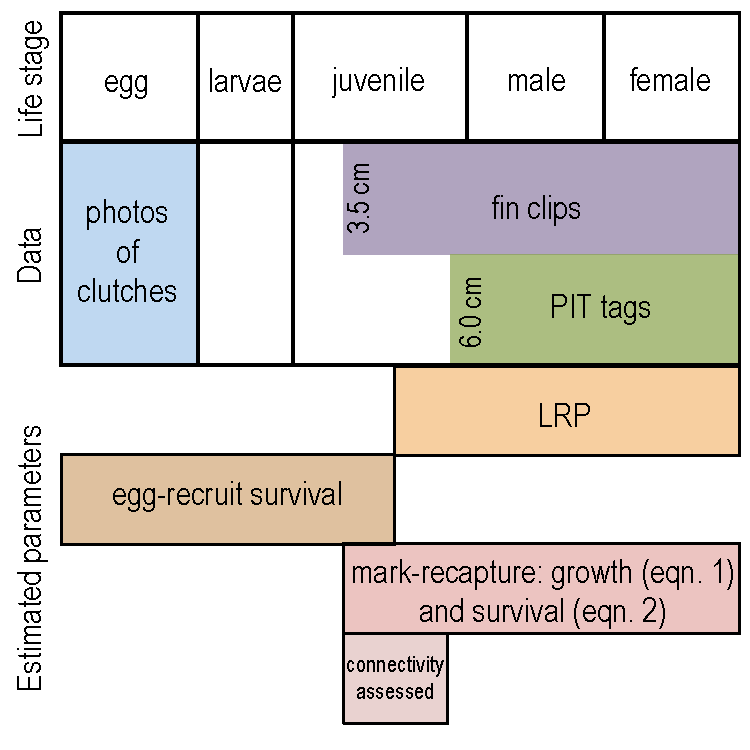
\includegraphics[width = 1.0\textwidth]{\detokenize{../Plots/Schematic/Schematic.pdf}}
	\caption{Here, we show the data collected for fish at each life stage (life stage boxes are not scaled by length of stage) and how the empirical data fit into our parameter and metric calculations. \label{FIG_Schematic}} % MAKE CAPTION BETTER! MAKE SCHEMATIC BETTER TOO!
\end{figure}

% Here, we estimate lifetime recruit production (LRP) as the number of surviving recruits a recruit-sized individual is expected to produce over its remaining lifetime. We find LRP by multiplying lifetime egg production (LEP) - the total number of eggs produced by one individual starting at the recruit stage (CITATIONS) - by the survival of an egg to the recruit stage ($S_e$):

% \begin{equation}
% \text{LRP} = \text{LEP} * S_e. \label{EQN_LRP}
% \end{equation}

% For a metapopulation to persist, at least one patch needs to achieve replacement, where the number of individuals entering the population balances those lost to mortality or emmigration \citep{burgess2014beyond, hastings_persistence_2006}. In many marine populations, including our focal system, exchange among patches occurs primarily at the larval stage (CITATIONS) so we can ignore emigration and only assess how far offspring travel before recruiting to a patch. We represent dispersal through a dispersal kernel and a connectivity matrix, where

% In our focal system, adults do not move among patches so we do not need to consider emmigration and only need to assess whether fish produce enough offspring that survive to recruitment to be able to replace themselves and where those offspring travel within the metapopulation. We consider three primary metrics to assess whether and how the population is persistent: 1) lifetime production of recruits, to assess whether the population has enough surviving offspring to achieve replacement 2) self-persistence, to assess whether any individual patches would be able to persist in isolation without any input from other patches, and 3) network persistence, to assess whether the metapopulation is persistent as a connected unit. We explain each metric below in detail. % Reference the section with \ref?

%% TEXT FROM INTRO TO INCORPORATE IF RELEVANT
% For any population to persist, individuals must on average replace themselves during their lifetimes. In non-spatially structured populations, we use criteria such as the average number of recruiting offspring contributed by each individual during its life (called $R_0$ when the population is age-structured and density-independent) or the growth rate of the population (such as the dominant eigenvalue $\lambda$ of an age-structured Leslie matrix) \citep{caswell_matrix_2001, burgess2014beyond}. To assess replacement, metrics must take into account the demographic processes across the whole life cycle, including how likely individuals are to survive to the next age or stage, their expected fecundity at each stage, and the survival of any offspring produced to recruitment. 

% In a spatially-structured population, persistence still requires replacement but in addition to assessing whether the reproductive output and survival of a population is sufficient, we must also consider how the offspring are distributed across space. The spread of offspring is often described using dispersal kernels, probability density functions that give the relative number of settlers with increasing distance from the origin patch \citep[e.g.][]{bode2018estimating}. Connectivity can also be described using a connectivity matrix, where entries give the probability of dispersing from one patch to another, either found by discretizing the dispersal kernel or through direct estimates of pairwise exchange among patches (choose some examples to cite). A long-held paradigm suggested that marine larvae were well-mixed and dispersed far on ocean currents \citep{roughgarden_recruitment_1988}, suggesting widespread connectivity. With the ability to estimate connectivity through natural tags such as otolith microchemistry or genetics and the realization that larvae can alter their dispersal through behavior \citep[e.g.][]{morgan_nearshore_2009}, however, the paradigm is shifting and local persistence of marine populations is seeming more possible. 

\subsection*{Study system}

We focus on a tropical metapopulation of yellowtail clownfish (\textit{Ampiprion clarkii}, Fig.\ \ref{FIG_Map_and_photo}c) in the Philippines. Like many clownfish species, yellowtail clownfish have a mutualistic relationship with anemones, where small colonies of fish live \citep{buston2003social, fautin1992field}. Yellowtail clownfish are protandrous hermaphrodites and maintain a size-strutured hierarchy; within an anemone, the largest fish is the breeding female, the next largest is the breeding male, and any smaller fish are non-breeding juveniles. The fish on an anemone maintain a strict social and size hierarchy \citep{buston2003social}, with fish moving up in rank to become breeders only after the larger fish have died or left. In the tropical patch reef habitat of the Philippines, yellowtail clownfish spawn once per lunar month from November to May, laying clutches of benthic eggs that the parents protect and tend \citep{ochi1989mating, holtswarth2017fecundity}. Larvae hatch after about six days and spend 7-10 days in the water column before returning to reef habitat to settle in an anemone \citep{fautin1992field}.

% % Other possible life histories in temperate areas or depending on the density of anemones
% \cite{hattori1991life}: different life history pathways found in population of \textit{A. clarkii} in Japan in area where they are the only anemonefish:
% \cite{ochi1989mating}: p.258: could be differences in the mating system/behavior of clownfish depending on how dense the host anemones are in the habitat and how costly it is to move between them; \textit{A. clarkii} in temperate areas off coast of Japan "showed many differences in behavior and morphology in comparison with conspecifics and othre anemonefishes from the primary habitats (coral reefs)."

Clownfish are particularly well-suited to metapopulation studies due to their limited movement as adults and clearly patchy habitat. Once fish have settled, they tend to stay within close proximity of their anemones [XX meters, CITATION]. This makes fish easier to relocate for mark-recapture studies and simiplifies the exchange between patches to only the dispersal during the larval phase. Patches, whether considered to be the reef patch or the anemone territory of the fish, are clearly discrete and easily delineated, which makes determining the spatial structure of the metapopulation clear. Additionally, clear patches make it easier to assess how much of the site has been surveyed. These simplifying characterstics in habitat and fish behavior make clownfish and other similarly territory-based reef fish useful model systems for studies of metapopulation dynamics and persistence \citep[e.g.][]{buston2013marine, salles_coral_2015, johnson2018integrating}. Our focal species of yellowtail clownfish tends to behave more like larger reef fishes, with territories that can extend beyond single anemones (CITATION) and strong enough swimming skills that movement between patch reefs is possible though unusual (CITATION), than the smaller clownfish \textit{A. percula} commonly used in previous metapopulation studies \citep[e.g.][]{buston2011probability, salles_coral_2015}.

\paragraph*{Field data collection}

We focus on a set of seventeen patch reef sites spanning approximately 30 km along the western coast of Leyte island in the Philippines (Fig.\ \ref{FIG_Map_and_photo}a). The sites consist of rocky patches of coral reef and are separated by sand flats (Fig.\ \ref{FIG_Map_and_photo}b). Previous work using genetic isolation by distances estimated that yellowtail clowfish larvae have a dispersal spread of about 10 km \citep[range 4-27 km,][]{pinsky2010using}, so our sites were selected to cover and exceed that range. On the north edge, the sites are isolated from nearby habitat with no substantial reef habitat for at least 20 km. % Pinsky et al. 2010 paper: (4–27 km with median 11 km)

\begin{figure}[H] % Map + clownfish photo
	\centering
	\includegraphics[width = 1.0\textwidth]{\detokenize{../Plots/FigureDrafts/Map_and_photo.pdf}}
	\caption{a) A map of the sites along the coast of Leyte in the Philippines. b) A zoomed-in map of Palanas and Wangag to show anemone arrangement for anemones occupied by \textit{A.\ clarkii} (green) or unoccupied by clownfish (green). c) An example anemone occupied by \textit{A.\ clarkii} in a typical habitat at the sites.  \label{FIG_Map_and_photo}} 
\end{figure}

Since 2012, we have sampled fish and habitat at most of the sites annually (Table \ref{APP_TAB_PercHabSampled}). During sampling, divers using SCUBA and tethered to GPS readers swam the extent of each site. Divers visited each anemone inhabited by yellowtail clownfish, tagging the anemone to be able to track anemones through time. At each anemone, the divers attempted to catch all of the yellowtail clownfish 3.5 cm and larger, taking a small tail fin-clip from each for use in genetic analysis, measuring the fork length, and noting the tail color (as an indicator of life stage). Starting in the 2015 field season, fish 6.0 cm and larger were also tagged with a passive integrated transponder (PIT) tag, unless already tagged. Divers also looked for eggs around each anemone and measure and photographed any clutches found. In total, we took fin clips from XX fish and PIT-tagged XX fish across all years and sites combined, with an average of XX fish clipped and XX fish tagged per year.

%\paragraph*{Genotyping and parentage analysis}
\paragraph*{Parentage analysis and dispersal kernel}  % Check with Katrina/Michelle that this captures the highlights and includes the right references

We digested extracted genomic DNA from our tissue samples using the ddRADseq protocol \citep{peterson2012double}, filtered the sequences with the bioinformatics pipeline dDocent \citep{puritz2014ddocent}, and called singled nucleotide polymorphisms (SNPs) using the program FreeBayes (\textit{is there a citation for this?}). In total, we genotyped XX fish. We used the SNPs to identify parent-offspring matches with the software program COLONY2 \citep{wang2012computationally} \citep[details on genotyping and parentage analysis in][]{catalanoInPrepconnectivity}.

Using the method described in \citep{bode2018estimating}, we fit a distance-based dispersal kernel \citep{catalanoInPrepconnectivity}, where the relative dispersal is a function of distance $d$ as measured in kilometers and parameters $\theta$ and $k_d$, which control the shape and scale of the kernel:
\begin{equation}
p(d) = e^k e^{-(e^k d)^\theta}. \label{EQN_DispKernel}
\end{equation}
We use a Laplacian dispersal kernel with shape parameters $\theta = 1$ and scale parameter $k_d = -1.84$ (Fig.\ \ref{FIG_ParameterInputs}a, estimated in \citep{catalanoInPrepconnectivity}).

The dispersal kernel is estimated using fish that have already recruited to a population and survived to be sampled so it gives the relative amount of dispersal given that a fish recruits somewhere, not the probability that a released larva will travel a particular distance. To find the probability of fish dispersing among our sites, we numerically integrate the dispersal kernel (eqn.\ \ref{EQN_DispKernel}) using the distance from the middle of the origin site to the closest and farthest bounds of the destination site as the upper and lower bounds. For example, the probability of dispersal from site A to B, where $d_1$ is the distance from the middle of A to the closest edge of B and $d_2$ is the distance from the middle of A to the far edge of B, is:
\begin{equation} % might not need this equation...
p_{A, B}(d) = \int_{d_1}^{d_2} e^k e^{-(e^k d)^\theta}  dd. \label{EQN_integratingDK}
\end{equation}

\subsection*{Estimating inputs from empirical data} % Which should come first, this section or the one about persistence metrics?

% \paragraph*{Defining recruit and census stage} % Not quite sure where to put this section... or if it should even be it's own section

% When assessing persistence, it is important to consider mortality and reproduction that occurs across the entire life cycle to determine whether an individual is replacing itself with an individual that reaches the same life stage \citep{burgess2014beyond}. We define a recruit to be a juvenile individual that has settled on the reef within the previous year; lifetime egg production assesses how many offspring an individual recruit is likely to produce in its lifetime from that point forward and egg-recruit survival gives us the fraction of those eggs that will survive to reach the recruit stage (Fig.\ \ref{FIG_Schematic}). In theory, it should not matter exactly how we define recruit so long we use that definition in our calculations of both egg-recruit survival and LEP. In our system it is straighforward to calculate LEP from any point but it is not possible to change our estimate of egg-recruit survival to allow different definitions of recruit: we do not have enough tagged recruits to reliably estimate survival to different recruit sizes. Instead, we choose the mean size of offspring matched in the parentage study as our best estimate of the size of a recruit ($\text{size}_\text{recruit}$) and test sensitivity to different sizes within the range of sizes that the recruit stage covers (Table \ref{TAB_Params}).

\paragraph*{Growth and survival: mark-recapture analyses}

We mark fish through both genetic samples and PIT tags, allowing us to estimate growth and survival through mark-recapture. After matching up recaptures of the same fish identified by genotype or tag, we have a set of encounters of XX marked fish that includes size and stage at each capture time.

For growth, we estimate the parameters of a von Bertalanffy growth curve \citep{fabens1965properties} in the growth increment form relating the length at first capture $L_t$ to the length at a later capture $L_{t+1}$ \citep{hart2009estimating}, where $L_\infty$ is the average asymptotic size across the population and $K$ controls the rate of growth: %check that I actually defined those well... % in the growth increment form (according to Hart and Chute) - need to actually get a copy of the Fabens paper, doesn't seem to be available on Google Scholar

\begin{equation} \label{EQN_VBL} 
\begin{split}
L_{t+1} & = L_t + (L_\infty - L_t)[1 - e^{(-K)}] \\
 & = e^{(-K)}L_t + L_\infty[1 - e^{(-K)}].
\end{split}
\end{equation}

We see from eqn.\ \ref{EQN_VBL} that we would expect the first length $L_t$ and the second length $L_{t+1}$ to be related linearly \citep{hart2009estimating}. From the slope $m = e^{(-K)}$ and y-intercept $b =  L_\infty[1 - e^{(-K)}]$, we can estimate the von Bertalanffy parameters, such that $K = -\ln m$ and $L_\infty = \frac{b}{(1-m)}$. We use the first and second capture lengths for fish that were recaught after a year (within 345 to 385 days) to estimate $L_\infty$ and $K$. We have some fish that were recaptured multiple times so we randomly select only one pair of recaptures from each to use in estimating the parameters, then repeat this process 1000 times to generate a distribution. 

We use the full set of marked fish to estimate annual survival $\phi$ and probability of recapture $p_r$ using the mark-recapture program MARK implemented in R \citep{RMark_Laake2013}. We consider several models with year, size, and site effects on the probability of survival and year and size effects on the probability of recapturing a fish on a log-odds scale (see full list in Table \ref{APP_TAB_MARKmodels}). For fish that are not recaptured in particular year, we estimate their size using our growth model (eqn.\ \ref{EQN_VBL}) and the size recorded or estimated in the previous year. Because fish are not well-mixed at our sites and instead stay quite close to their home anemones, we need to swim near an anemone to have a reasonable chance of capturing the fish on it. Therefore, we also consider a distance effect on recapture probability; we use the GPS tracks of divers to estimate the minimum distance between a diver and the anemone for each tagged fish in each sample year and include it as a factor in some of the models (Table \ref{APP_TAB_MARKmodels}).

\paragraph*{Fecundity}

We use a size-dependent fecundity relationship, determined using photos of egg clutches and females \citep{yawdoszynInPrepfecundity}, where the number of eggs per clutch ($E_c$) is exponentially related to the length in cm of the female ($L$) with size effect $\beta_l = 2.388$, intercept $b = 1.174$, and egg age effect $\beta_e = -0.6083$ dependent on if the eggs are old enough to have visible eyes: 
\begin{equation} % is this the best way of writing this?
\ln(E_c) = \beta_l\ln(L) + \beta_e[\text{eyed}] + b. \label{EQN_Fec}
\end{equation}
To get total annual fecundity $f$, we multiply the number of eyed eggs per clutch by the number of clutches per year $c_e = 11.9$, using the estimate from \cite{holtswarth2017fecundity}.

We only consider reproductive effort once the fish has reached the female stage and use the average size of first observation as female for recapture fish as the transition size $L_f$.

% We only consider reproductive effort once the fish has reached the female stage. Though the size at which a fish transitions to become a breeding female $L_f$ will depend on the size hierarchy in each particular colony [CITATION], we use the average size recaptured fish were first observed as female. 

% For comparison of numbers (from Clownfish\_SP\_Notes:) Moyer (1986): the individual observed for 11 years and thought to live to at least 13 was ”estimated to have contributed about 160,000 propagules in its lifetime,” spent 3 years as a functional male, then outlived 3 mates as a female; fertilized about 45,000 eggs during 3 years as a male, then spawned about 115,000 eggs as a female; fecundity estimate at this site (Miyake-jima in Japan) is 17,500 eggs/yr/female (from Bell (1976))

\paragraph*{Lifetime egg production}
We use an integral projection model (IPM) \citep[e.g.][]{rees2014building} to estimate the total number of eggs produced by one individual (lifetime egg production: LEP), starting at the recruit stage, when individuals have settled and survived to a size we can sample.

In an IPM, the state of the population at time $t$ is described by the distribution of the population over a continuous trait $z$, for which we use size: $n(z,t)$. The total number of individuals in the population at time $t$ is the integral of the size distribution over size from the lower size bound $L$ to the upper size bound $U$: $\int_L^U n(z,t) dz$. The population is projected forward with probability density functions, called the kernel, that describe the survival, growth, and reproductive output of existing individuals into the next time step. 

We initalize the IPM with one recruit-sized individual ($\text{size}_\text{recruit}$): $n(t=0) = n(\text{size}_\text{recruit}, 0)$, then use a kernel with the size-dependent survival and growth functions described above to project forward for 100 time steps. This gives us the size distribution at each time step, which represents the probability that the individual has survived and grown into each of the possible size categories. The probability that the individual is still alive and of any size decreases as the time steps progress; by using a large number of steps, we are able to avoid arbitrarily setting a maximum age and instead let the probabilities become essentially zero. 

We then multiply each size-distribution vector $v_z$ in the matrix by the size-dependent fecundity function described above (eqn.\ \ref{EQN_Fec}) to get the total number of eggs produced at each time step. To get the total number of eggs one individual is likely to produce in its lifetime, we then sum across all time steps in the individual's potential life.  

\begin{equation} % I'm not sure this is quite right...
\text{LEP} = \Sigma_{t=0}^{t=100} \Sigma_{z=L}^{z=U} v_z,t f_z. \label{EQN_LEP}
\end{equation}

\paragraph*{Survival from egg to recruit}

We use a method similar to that in \cite{johnson2018integrating}, using parentage matches to estimate the number of surviving recruits produced by genotyped parents, to estimate survival from egg to recruit ($S_e$). We estimate the number of eggs produced by genotyped parent fish by multiplying the number of genotyped parents ($N_g = XXX$) by the expected lifetime egg production for a fish of parent size ($LEP_p$), using LEP calculated for a fish of 6 cm, the minimum size to be considered a parent in the parentage analysis \citep{catalanoInPrepconnectivity}. To get an estimate of the total number of recruits these parents might have produced, we scale the number of offspring we find that match to parents ($R_m = XX$, "tagged" recruits because they are able to be genetically matched back to their parents) by the proportion of our site habitat we sampled cumulatively across all sampling years ($P_h = 0.34$) and the probability of capturing a fish if we sample its anemone ($P_c$) (see \ref{APP_SEC_ProbHabSampled}, \ref{APP_SEC_ProbR} for details on $P_h$ and $P_c$ estimates, respectively). Our sites do not encompass all of the area where an offspring might disperse and settle, so we also scale the estimated recruited offspring by the proportion of the total dispersal kernel area from each of our sites covered within our sampling region ($P_d$) to account for offspring from our parents that might have settled outside our sampling areas (details in \ref{APP_SEC_PropDispKernelSampled}). We then take this scaled number of estimated "tagged" recruits and divide it by the number of genetically tagged eggs produced by the genotyped parents to get an estimate of egg-recruit survival:

\begin{equation}
S_e = \frac{\frac{R_m}{P_h P_c P_d}}{N_g \text{LEP}_p}. \label{EQN_EggRecruitSurv}
\end{equation}

% We estimate survival $S_e$ from egg to recruit using the number of recruited offspring we can match back to genotyped parents as surviving individuals from genetically "tagged" eggs in a method similar to that in \cite{johnson2018integrating}. We estimate the number of eggs produced by genotyped parent fish by multiplying the number of genotyped parents ($N_g = 913$) by the expected lifetime egg production of a parent fish $LEP_p$, using LEP calculated starting with an individual of 6 cm. We make the assumption that all recruited offspring originating from the genotyped parents end up in one of the sites we sample and estimate the total number of offspring that survive to recruit $R_t$ by dividing the number of offspring matches we find ($R_m = 90$) by the proportion of our site habitat we sample cumulatively across all sampling years ($P_h = 0.34$) and the probability of capturing a fish if we sample an anemone $P_c$ (see \ref{APP_SEC_ProbHabSampled}, \ref{APP_SEC_ProbR} for details on $P_h$ and $P_c$ estimates, respectively). Our estimated survival from egg to recruit is the number of tagged recruits divided by the number of tagged eggs produced:

% \begin{equation}
% S_e = \frac{\frac{R_m}{P_h P_c}}{N_g \text{LEP}_p}. \label{EQN_EggRecruitSurv}
% \end{equation}

\paragraph*{Accounting for density-dependence}  % Should this be its own section or part of the survival from egg to recruit?

Ideally we would assess persistence metrics when the population is at low abundance and not limited by density-dependence, so we attempt to account for the effects of density-dependence in the early life stages when it is likely strongest. Clownfish have strong social hierarchies and in other clownfish species, juveniles that have already settled on an anemone will prevent others from settling there as well \citep{buston2003forcible}. Each anenome, therefore, can only house one settling clownfish, so having anemones already occupied by \textit{A. clarkii} reduces the survival from egg to recruit if potential settlers get evicted by resident juveniles when they try to settle. We attempt to account for this density-dependent mortality by multiplying our estimate of settling recruits (the numerator of eqn.\ \ref{EQN_EggRecruitSurv}) by the proportional increase ($\text{DD}$) in unoccupied anemones at our sites if all of the \textit{A. clarkii} anemones were unoccupied, where $p_\text{APCL}$ is the proportion of anemones occupied by \textit{A. clarkii} and $p_\text{UNOC}$ is the proportion of unoccupied anemones: $\text{DD} = \frac{(p_\text{UNOC} + p_\text{APCL})}{p_\text{UNOC}}. We present results both with and without this density-dependence modification.


% \paragraph*{Defining recruit and census stage} % Not quite sure where to put this section... or if it should even be it's own section

% When assessing persistence, it is important to consider mortality and reproduction that occurs across the entire life cycle to determine whether an individual is replacing itself with an individual that reaches the same life stage \citep{burgess2014beyond}. We define a recruit to be a juvenile individual that has settled on the reef within the previous year; lifetime egg production assesses how many offspring an individual recruit is likely to produce in its lifetime from that point forward and egg-recruit survival gives us the fraction of those eggs that will survive to reach the recruit stage. In theory, it should not matter exactly how we define recruit so long we use that definition in our calculations of both egg-recruit survival and LEP. In our system it is straighforward to calculate LEP from any point but it is not possible to change our estimate of egg-recruit survival to allow different definitions of recruit: we do not have enough tagged recruits to reliably estimate survival to different recruit sizes. Instead, we choose the mean size of offspring matched in the parentage study as our best estimate of the size of a recruit ($\text{size}_\text{recruit}$) and test sensitivity to different sizes within the range of sizes that the recruit stage covers (Table \ref{TAB_Params}).

% \paragraph*{Probability of dispersal}

% We use a distance-based dispersal kernel, estimated in other work using parent-offspring matches from our genetic data \citep{catalanoInPrepconnectivity} using the method described in \cite{bode2018estimating}. The relative dispersal is a function of distance $d$ as measured in kilometers and parameters $\theta$ and $k_d$, which control the shape and scale of the kernel:
% \begin{equation}
% p(d) = e^k e^{-(e^k d)^\theta}. \label{EQN_DispKernel}
% \end{equation}
% We use a Laplacian dispersal kernel with shape parameters $\theta = 1$ and scale parameter $k_d = -1.84$ (Fig.\ \ref{FIG_ParameterInputs}a, estimated in \citep{catalanoInPrepconnectivity}).

% The dispersal kernel is estimated using fish that have already recruited to a population and survived to be sampled so it gives the relative amount of dispersal given that a fish recruits somewhere, not the probability that a released larva will travel a particular distance. To find the probability of fish dispersing among our sites, we calculate the distance between the middle of each site to the closest and farthest edge of each other site, then use the distances as upper and lower bounds when integrating eqn. \ref{EQN_DispKernel}, which we do numerically. For example, the probability of dispersal from site A to B, where $d_1$ is the distance from the middle of A to the closest edge of B and $d_2$ is the distance from the middle of A to the far edge of B, is:

% \begin{equation} % might not need this equation...
% p_{A, B}(d) = \int_{d_1}^{d_2} e^k e^{-(e^k d)^\theta}  dd. \label{EQN_integratingDK}
% \end{equation}

\paragraph*{Estimated abundance over time}

We also consider trends in abundance of breeding females at each site over time to compare to our replacement-based estimates of persistence. Similarly to as we do for offspring, we scale up the number of females caught at each site $i$ in each sampling year $t $by the proportion of habitat sampled in that site and year $P_{h_{i,t}}$ and by the probability of capturing a fish $P_c$:
\begin{equation}
\text{\# females}_{i,t} = \frac{\text{\# females captured}_{i,t}}{P_{h_{i,t}}P_c}. \label{EQN_FemaleAbundance}
\end{equation}

We then fit a linear model through the time series for each site and the population overall to assess whether the slope $m$ over time indicates growth, decline, or stability in abundance:
\begin{equation}
\text{\# females} = m*\text{year} + b. \label{EQN_AbundanceLM}  % There has got to be a better way to write this!
\end{equation}

% \subsection*{Persistence metrics}

% For a metapopulation to persist, at least one patch needs to achieve replacement, where the number of individuals entering the population balances those lost to mortality or emmigration \citep{burgess2014beyond, hastings_persistence_2006}. In our focal system, adults do not move among patches so we do not need to consider emmigration and only need to assess whether fish produce enough offspring that survive to recruitment to be able to replace themselves and where those offspring travel within the metapopulation. We consider three primary metrics to assess whether and how the population is persistent: 1) lifetime production of recruits, to assess whether the population has enough surviving offspring to achieve replacement 2) self-persistence, to assess whether any individual patches would be able to persist in isolation without any input from other patches, and 3) network persistence, to assess whether the metapopulation is persistent as a connected unit. We explain each metric below in detail. % Reference the section with \ref?

% % Should I include some sort of discussion of time series?


% \paragraph*{Lifetime production of recruits}

% To assess whether individuals at our focal patches produce enough offspring that survive to become recruits themselves, we find the estimated number of recruits an individual recruit will produce over its lifetime (lifetime recruit production: LRP) by multiplying LEP by the estimated survival from egg to recruit $S_e$:
% \begin{equation}
% \text{LRP} = \text{LEP} * S_e. \label{EQN_LRP}
% \end{equation}
% If $LRP \geq 1$, the population has the possibility for replacement; indviduals produce enough surviving offspring, before taking into account the probability of dispersal. If $LRP < 1$, the individuals are not replacing themselves and the population cannot persist without input from outside patches.

% \paragraph*{Self-persistence}

% A patch is able to persist in isolation (self-persistent) if individuals produce enough offspring (LEP) that disperse back to the natal patch and survive to recruitment to be able to replace themselves (LR): $\text{LEP} \times \text{LR} \geq 1$ \citep{burgess2014beyond}. Our dispersal kernel represents the probability that a recruit disperses a distance given that it recruits somewhere, rather than the probability of a larva dispersing and recruiting to a particular patch, which implicitly encompasses mortality from egg to recruitment. We modify the equation to fit our data and include survival from egg to recruit to assess whether a particular patch $i$ is self-persistent: 
% \begin{equation}
% \begin{split}
% SP_i &= \text{LEP} \times \frac{\text{recruits}}{\text{egg}} \times \frac{p_{i,i} \times \text{\# recruits from patch i}}{\frac{\text{recruits}}{\text{egg}} \times \text{\# eggs produced by patch i}} \\ 
% %SP_i &= \text{LEP} \times S_e \times \frac{p_{i,i} \times \text{\# recruits from site $i$}}{S_e \times \text{\# eggs produced by patch $i$}} \\
% SP_i &= \text{LEP} \times S_e \times p_{i,i}. \label{EQN_SP}
% \end{split}
% \end{equation}
% A patch is self-persistent if $\text{SP} \geq 1$. If at least one patch is self-persistent, the metapopulation as a whole is persistent as well \citep{hastings_persistence_2006, burgess2014beyond}.

% \paragraph*{Realized connectivity matrix and network persistence}
% We find the probabilities of a recruit dispersing between each set of sites ($p_{i,j}$) by integrating the dispersal kernel (eqn.\ \ref{EQN_DispKernel}) over the distance between each set of sites. We then create a realized connectivity matrix $C$ by multiplying the dispersal probabilities by the expected number of recruits an individual produces: $C_{i,j} = \text{LRP} \times p_{i,j}$ \citep{burgess2014beyond}. The diagonal entries of $C$, where the origin and destination are the same sites, are the values of self-persistence we calculate above. 

% Network persistence requires that the largest real eigenvalue of the realized connectivity matrix $\lambda_C$ be greater than $1$: $\text{NP} = \lambda_C > 1$ \citep[e.g.][]{hastings_persistence_2006, white_population_2010, burgess2014beyond}.

\paragraph*{Incorporating uncertainty}
To represent the uncertainty in our estimates of the parameters that go into calculating our persistence metrics, we calculate each metric 1000 times, pulling each parameter from a distribution or range. In our results, we show the range of values of each persistence metric as well as the value with our best estimate of each parameter. 

For the dispersal kernel, we keep the shape parameter $\theta$ constant and pull the scale parameter $k_d$ from a set capturing the 95\% confidence intervals, which was produced during kernel estimation in \cite{catalanoInPrepconnectivity}. To capture uncertainty in the size of a recruit $\text{size}_\text{recruit}$, and therefore the transition of mortality being captured by egg-recruit survival to being captured by LEP, we pull from a uniform distribution over the range of fish sizes (3.5 - 6.0 cm) considered as offspring in the parentage analyses \citep{catalanoInPrepconnectivity}. We include uncertainty in the size of transition to a breeding female $L_F$ by pulling from the set of sizes observed in the data for fish at their first recapture as a female. For the von Bertalanffy growth parameters $L_\infty$ and $K$, we pull from the full set of estimates using different combinations of recapture pairs for fish recaptured more than twice. For uncertainty in adult survival, we pull from a normal distribution generated using the uncertainty estimated in the mark-recapture analysis for both the intercept $b_\phi$ and the size effect $b_a$.

To incorporate uncertainty in egg-recruit survival, we consider uncertainty in both the number of offspring assigned to parents $R_m$ during the parentage analysis and the probability of capturing a fish $P_c$, which affects how the captured assigned offspring are scaled up to account for fish uncaught. For the number of assigned offspring, we generate a set of values of number of assigned offspring using a random binomial, where the number of trials is the number of genotyped offspring (XX) and the probability of success on each trial is the assignment rate XX of offspring from the parentage analysis \citep{catalanoInPrepconnectivity}. To represent uncertainty in the probability of capturing a fish, we pull values from a beta distribution with parameters $\alpha_{P_c}$ and $\beta_{P_c}$, found using the mean and variance of capture probabilities estimated from recapture dives across sites and sampling seasons (details in \ref{APP_SEC_ProbR}). 

\section*{Results}

Our estimated abundance of females at each site over time is relatively constant [\textit{add some sort of actual analysis here}] (Fig.\ \ref{FIG_FthroughTime}), suggesting that our sample populations are stable over time.

\begin{figure}[H] %  abundance trends through time with some sort of time series analysis
	\centering
	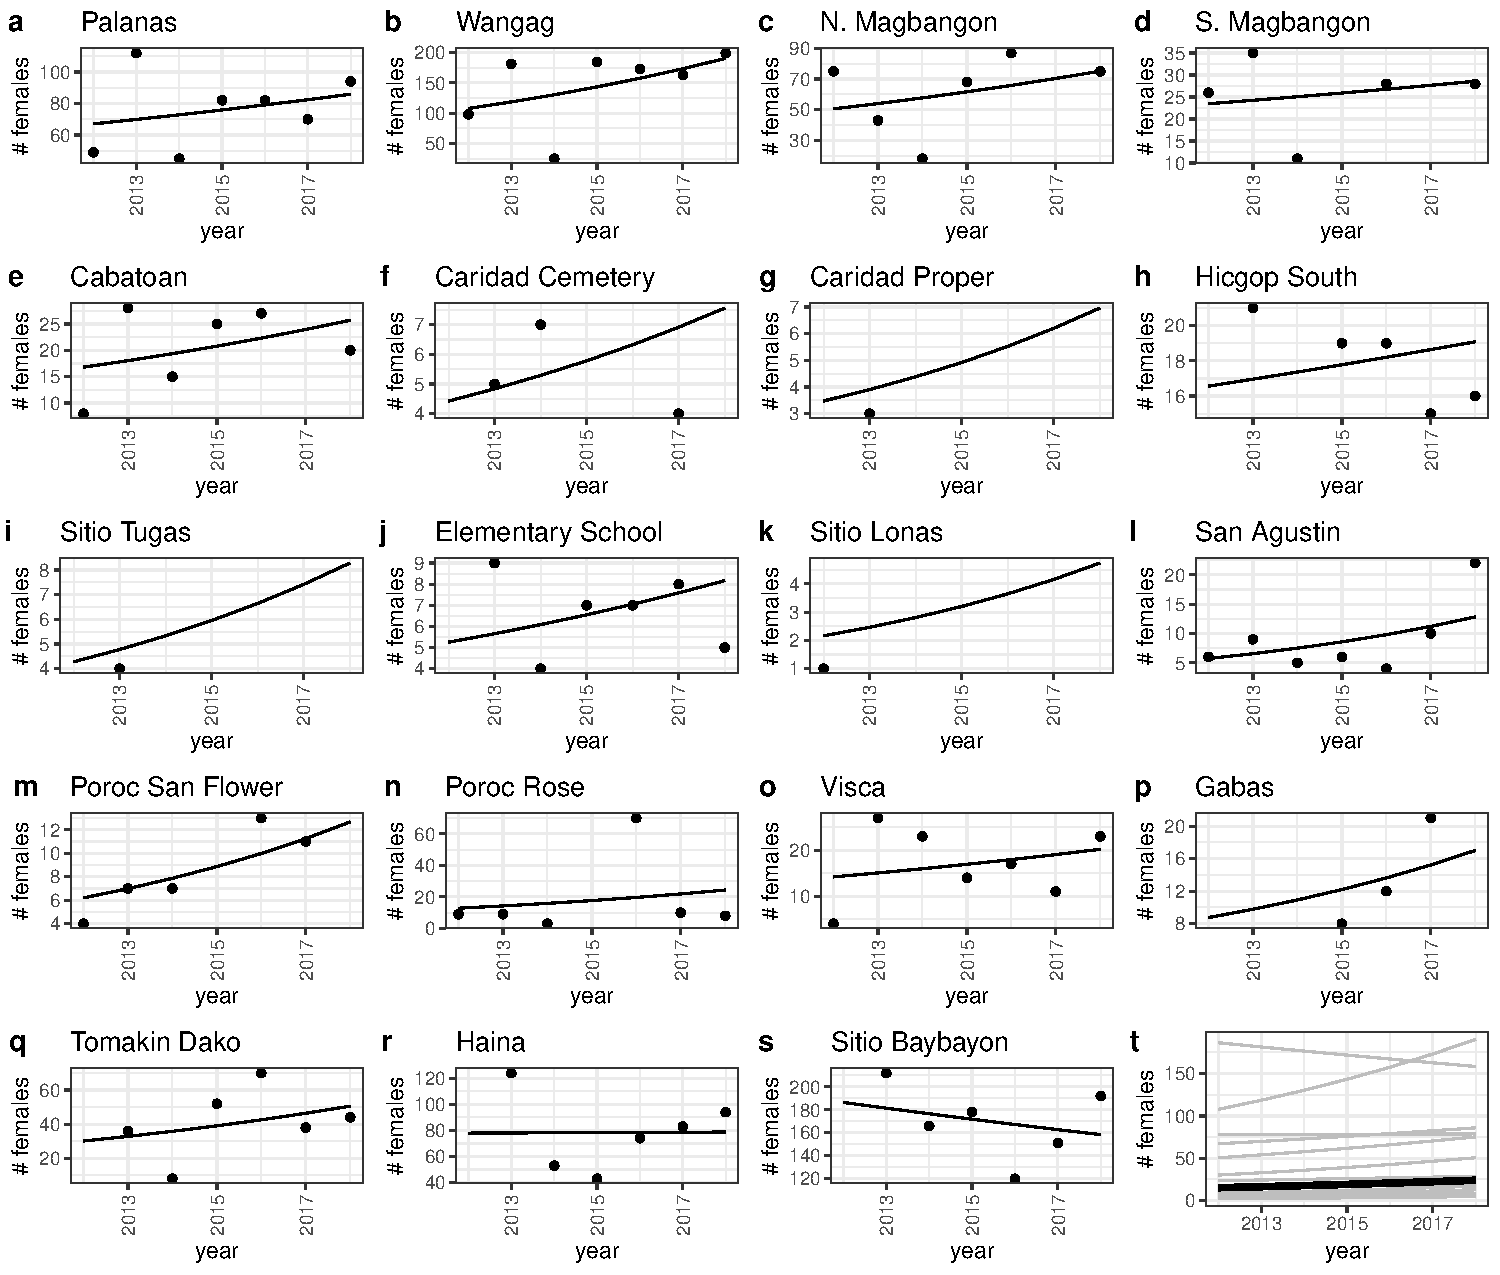
\includegraphics[width = 1.0\textwidth]{\detokenize{../Plots/FigureDrafts/Time_series_scaled_F_by_site_with_lines.pdf}}
	\caption{The estimated number of females at each site over the sampling years. The total number of females at each site was estimated by taking the number of females (fish $>$ 5 cm with the yellow pointed tail indicating female) captured at each site in each year and scaling up by the proportion of habitat sampled at that site that season (see \ref{APP_SEC_ProbHabSampled} for details) and by the average probability of capturing a fish (see \ref{APP_SEC_ProbR}). \label{FIG_FthroughTime}}
\end{figure}

From the mark-recapture analysis of tagged and genotyped fish, we estimate mean values of $L_\infty = 10.58 \text{cm}$ (range of estimates 10.39 - 10.75 cm) and $K = 0.928$ (range of estimates 0.854 - 1.025) for the von Bertalanffy growth curve parameters (Fig.\ \ref{FIG_ParameterInputs}b, Table \ref{TAB_Params}). For juvenile and adult (post-recruitment) survival on a log-odds scale, the best-fit model has a coefficient $b_a = 0.74 \pm 0.060$ SE for the effect of size and an intercept $b_\phi = -4.83 \pm 0.340$ SE. These results suggest that larger fish have higher annual survival, which is similar to survival estimates in other clownfish species (check Buston paper). The accompanying best-fit model for log-odds recapture probability has intercept $b_{p_r} = 17.93 \pm 0.858$ SE, size effect $b_1 = -1.816 \pm 0.080$ SE, and effect of diver distance from the anemone $b_2 = -0.171 \pm 0.021$ SE. The negative effect of both size and distance suggest that divers are less likely to recapture larger fish and those at anemones far from areas sampled, with the chance of recapturing an average-sized fish falling below 5\% if a diver stays farther than XX from its home anemone [add the recapture probability plots, like the survival one in Fig.\ \ref{FIG_ParameterInputs}, to the appendix and reference here.] 

We set the transition size to breeding female $L_f$ at 9.32 cm, the mean size of first female capture of recaptured fish (Fig. \ref{FIG_ParameterInputs}d). [\textit{Contextualize these values.}]

% Results about survival model that was previously in methods - need to work into existing results text
% The best-fit model using model selection with AICc has an effect $b_a$ of fish size on survival, and additive effects $b_1$ and $b_2$ of fish size and shortest distance to anemone on the probability of recapture:

% \begin{eqnarray}
% \log(\frac{\phi}{1-\phi}) &=& b_\phi + b_a\text{size} \\
% \log(\frac{p_r}{1-p_r}) &=& b_{p_r} + b_1\text{size} + b_2d. \label{EQN_Survival}
% \end{eqnarray}
% Assume I shouldn't talk about fecundity model results and dispersal kernel results here b/c they are done in other papers? Or should I? But put their parameters below for easy reference?

[\textit{Not sure where to put this table - kind of a methods/results hybrid, or if it should exist, but seems like it might be helpful. Need to clarify somewhere what kind of distributions are going into the uncertainty runs (drawn from data, uniform across a range, 95\% confidence bounds, etc.)}]
\begin{centering}
\begin{longtable}{|p{0.8in}|p{1.2in}|p{1.5in}|p{1in}|p{1.5in}|}
\hline 
\textbf{Parameter} & \textbf{Description} & \textbf{Best estimate} & \textbf{Range in uncertainty runs} & \textbf{Notes} \\ \hline
$k_d$ & scale parameter in dispersal kernel & -1.36 & -2.03 to -0.96 & estimated using methods in \cite{bode2018estimating} in Catalano et al.\ (in prep) \\ \hline
$\theta$ & shape parameter in dispersal kernel & 0.5 & NA & estimated using methods in \cite{bode2018estimating} in Catalano et al.\ (in prep) \\ \hline
$L_\infty$ & average asymptotic size in von Bertalanffy growth curve & 10.58 cm & 10.39 to 10.75 cm &  \\ \hline
$K$ & growth coefficient in von Bertalanffy growth curve &  0.928 & 0.854 to 1.025 & \\ \hline  
$b_\phi$ & intercept for adult survival & -4.83 & $\pm$ 0.340 standard error & \\ \hline
$b_a$ & size effect for adult survival & 0.74 & $\pm$ 0.060 standard error & \\ \hline
$b_{p_r}$ & intercept for recapture probability from mark-recapture analysis & 17.93 & $\pm$ 0.858 standard error & not used in persistence estimates \\ \hline
$b_1$ & size effect for recapture & -1.816 & $\pm$ 0.080 standard error & not used in persistence estimates \\ \hline
$b_2$ & distance effect for recapture & -0.171 & $\pm$ 0.021 standard error & not used in persistence estimates \\ \hline
$\text{size}_\text{recruit}$ & size (cm) of recruited offspring & mean of size of offspring in parentage analysis = 4.4 cm & 3.5 - 6.0 cm & \\ \hline
%$S_e$ & egg-recruit survival & & &  \\ \hline
%$E_c$ & eggs per clutch & depends on female size (eqn.\ \ref{EQN_Fec}) & & relationship from Yawdoszyn et al.\ (in prep) \\ \hline
$b_e$ & coefficient for eyed eggs & -0.608 & & Yawdoszyn et al.\ (in prep) \\ \hline
$b_l$ & size effect in eggs-per-clutch relationship & 2.39 & & Yawdoszyn et al.\ (in prep) \\ \hline
$b$ & intercept in eggs-per-clutch relationship & 1.17 & & Yawdoszyn et al.\ (in prep) \\ \hline
$L_f$ & size at transition to female & 9.32cm & 5.2 - 12.7cm & \\ \hline
$P_c$ & probability of capturing a fish & 0.56 & drawn from beta distribution with parameters $\alpha_{P_c} = 1.44$ and $\beta_{P_c} = 1.13$ & details in \ref{APP_SEC_ProbR} \\ \hline
\caption{}\label{TAB_Params}
\end{longtable}
\end{centering}

\begin{figure}[H] % demographic parameters: survival curve, growth curve, dispersal kernel, transition size to female 
	\centering
	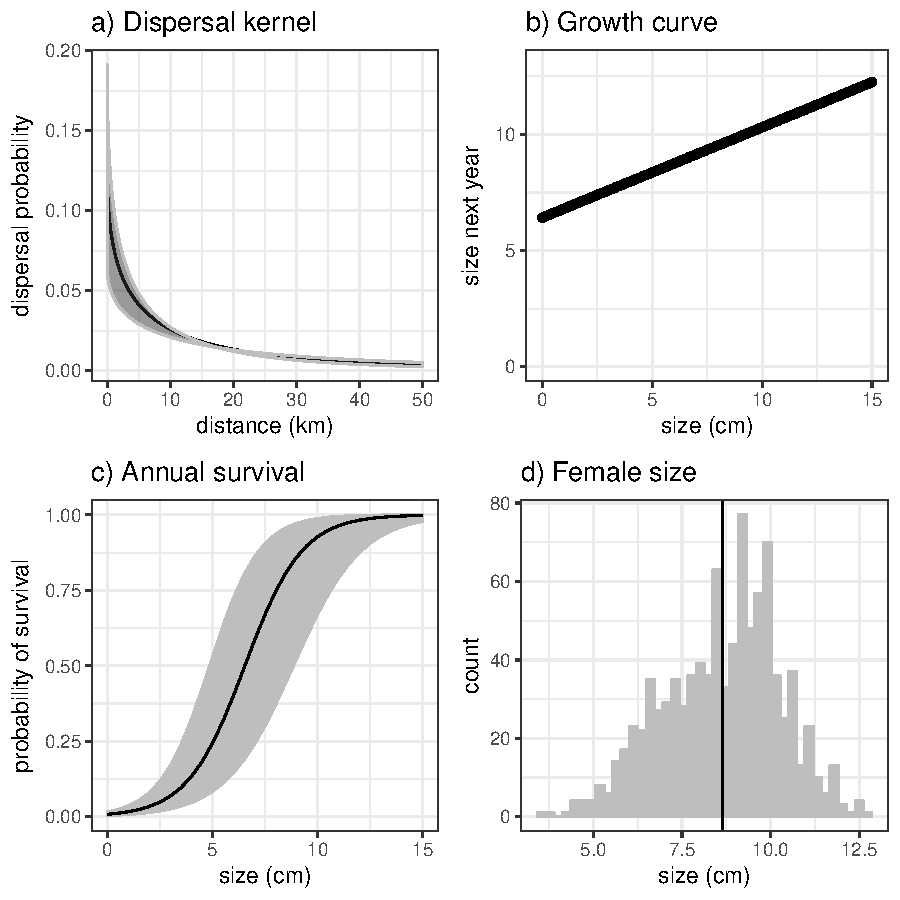
\includegraphics[width = 1.0\textwidth]{\detokenize{../Plots/FigureDrafts/Parameter_inputs.pdf}}
	\caption{Best estimates (solid black line) and range included for uncertainty (gray) for dispersal (a), growth (b), post-recruit survival (c), and size at female transition (d) parameters. \label{FIG_ParameterInputs}}
\end{figure}

Using our best estimates for growth, survival, and fecundity, we calculate a value of LEP for 10876, ranging from XX to XX when we consider uncertainty in the inputs (Fig.\ \ref{FIG_LEP_RperE_LRP}a). The size at recruitment - the cenusus point between egg-recruit survival and LEP - has the most effect on the value of LEP (Fig.\ \ref{APP_FIG_Uncertainty_LEP}), with higher values of LEP the higher the size of recruitment as less mortality is included before reaching reproductive sizes. 

We estimate egg-recruit survival $S_e$ to be 1.82e-05, ranging from XX to XX when we include uncertainty in the number of offspring assigned to parents and the probability of catching a fish (Fig.\ \ref{FIG_LEP_RperE_LRP}b). Uncertainty in the size of transition to breeding female $L_f$ has the largest effect on egg-recruit survival (Fig.\ \ref{APP_FIG_Uncertainty_RperE}); we only consider reproduction from females, to avoid double-counting, so the larger the transition size to female, the fewer tagged eggs we estimate were produced by genotyped parents and the higher egg-recruit survival. % REPHRASE THIS BETTER! THEN TALK ABOUT LRP - what that means for persistence potential.

We estimate lifetime recruit production, the product of LEP and $S_e$, to be 0.20, below the value of 1 necessary for replacement. This suggests that even without considering connectivity, the individuals at our sample populations do not produce enough offspring that survive to recruitment to replace themselves. When we consider uncertainty in our parameter estimates, we do see a few cases where LRP $>$ 1, but the majority are well below the threshold for replacement.

\begin{figure}[H] % LEP, recruits-per-egg, LRP shown with uncertainty, line for best estimate (using mean offspring size as recruit size)
	\centering
	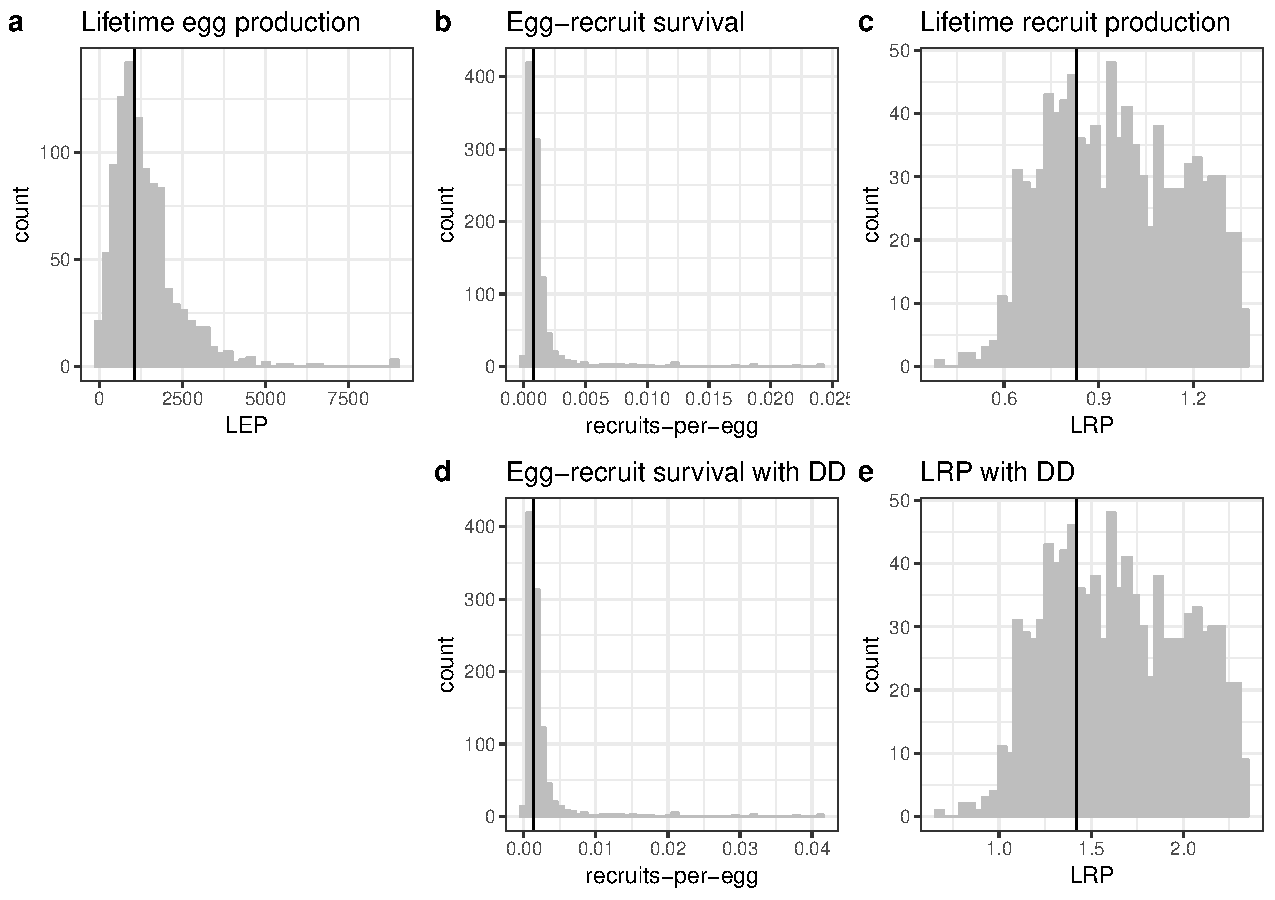
\includegraphics[width = 1.0\textwidth]{\detokenize{../Plots/FigureDrafts/LEP_RperE_LRP.pdf}}
	\caption{Estimates of a) LEP, b) egg-recruit survival, and c) LRP, showing the best estimate (black solid line) and range of estimates considering uncertainty in the inputs. \label{FIG_LEP_RperE_LRP}}
\end{figure}

We do not find any sites with self-persistence values $>$ 1, indicating that the site could persist in isolation. Given that our estimate of LRP does not suggest replacement and only a fraction of that recruitment stays at the natal site, this makes sense. We see the highest values of self-persistence at Haina ($\text{SP} = 0.024$) and Wangag ($\text{SP} = 0.010$), our two widest sites.

\begin{figure}[H] % SP with line for best estimate (using mean offspring size as recruit size)
	\centering
	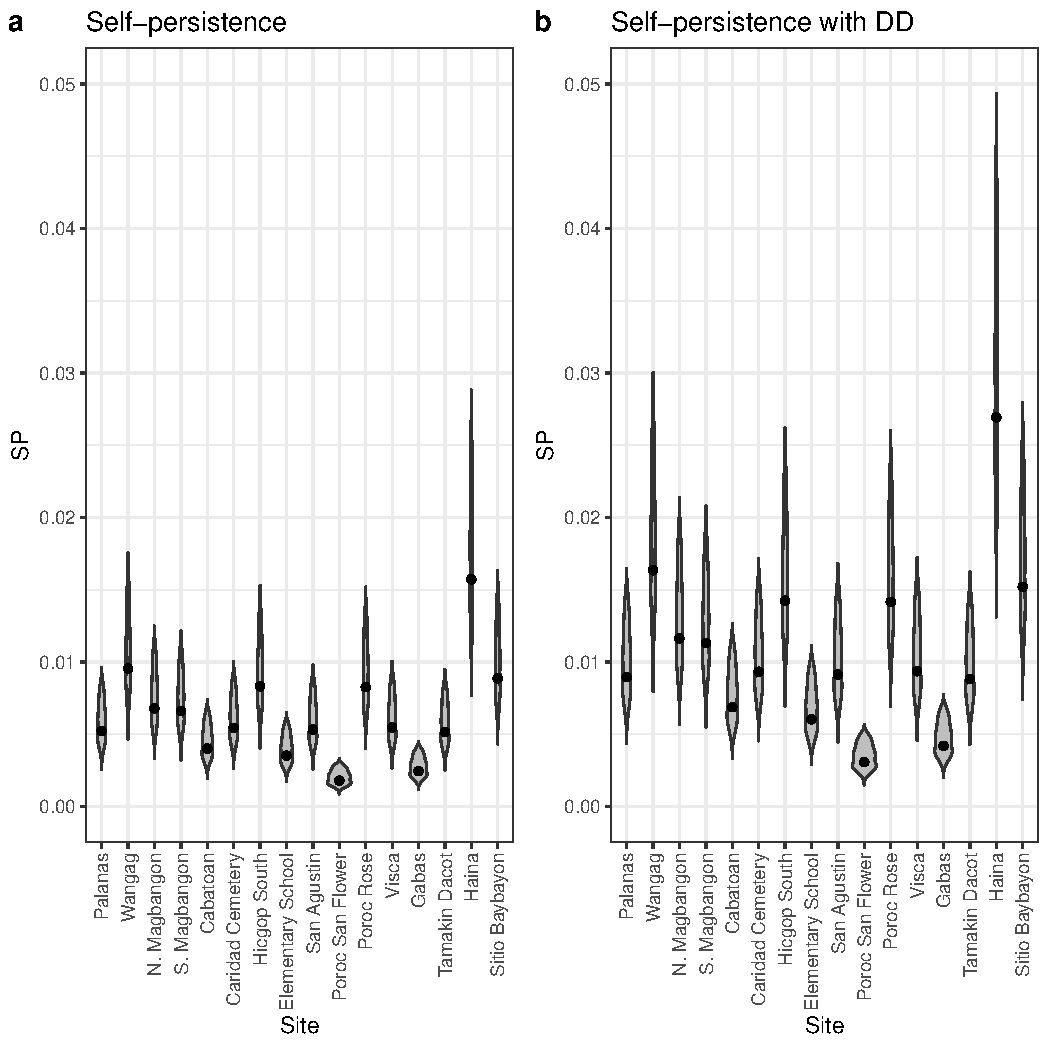
\includegraphics[width = 1.0\textwidth]{\detokenize{../Plots/FigureDrafts/SP_hists_by_site_noSLSTCP.pdf}}
	\caption{Values of self-persistence at each site, showing the best estimate (black point) and range of estimates considering uncertainty in the input paramters. No site reaches a value of SP $>$ 1, necessary to be self-persistent. \label{FIG_SP}}
\end{figure}

We also do not find evidence of network persistence; the dominant eigenvalue of the realized connectivity matrix $\lambda_c$ is 0.034, well below the value of 1 that indicates network persistence (Fig.\ \ref{FIG_NP_realizedCmat}a). We see that most of the connectivity occurs among the sites in the northern part of our sample area, from Palanas to Caridad Cemetery.

\begin{figure}[H] % NP with line for best estimate (using mean offspring size as recruit size), realized connectivity matrix for best estimate - should re-do without Sitio Lonas, Sitio Tugas, Caridad Proper!
	\centering
	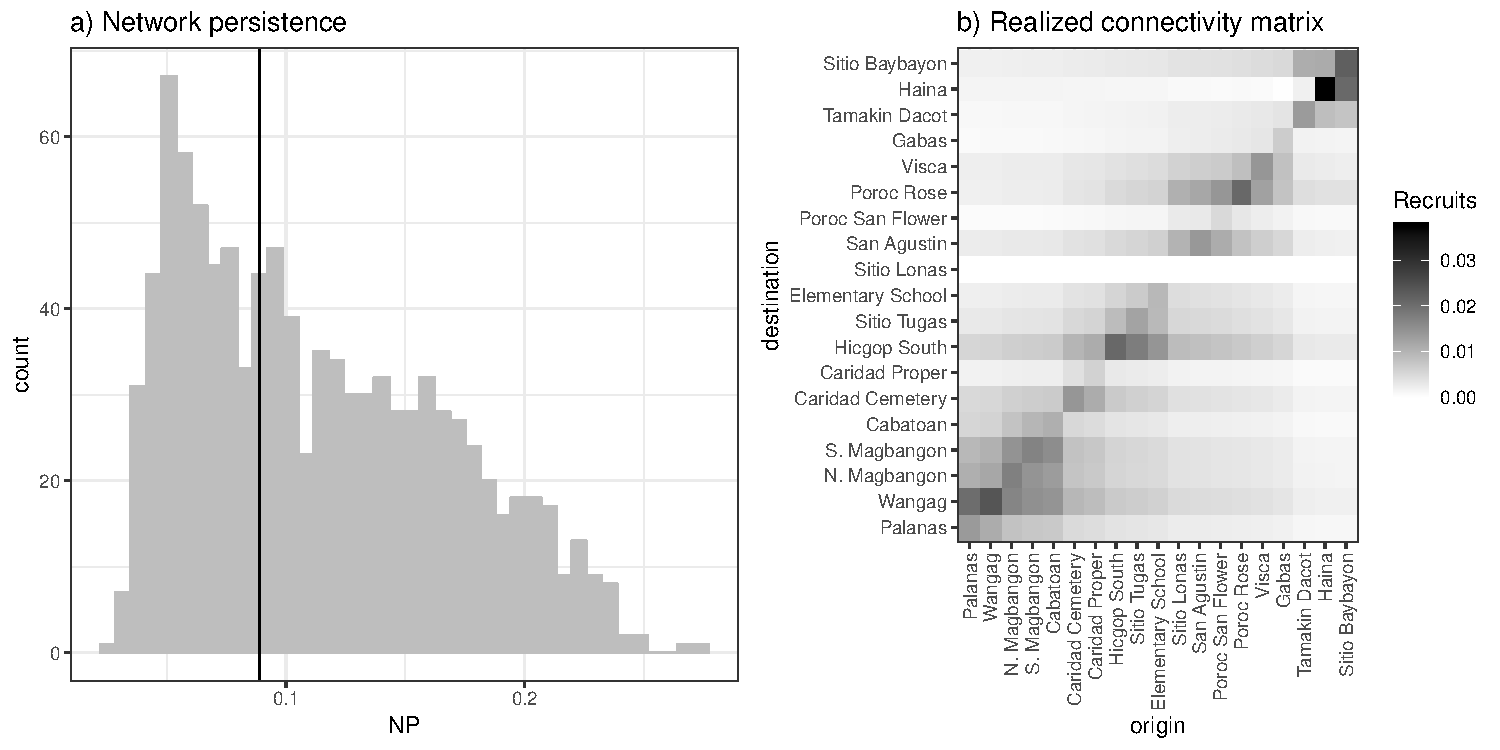
\includegraphics[width = 1.0\textwidth]{\detokenize{../Plots/FigureDrafts/NP_and_connMatrixR.pdf}}
	\caption{a) Network persistence values, showing the best estimate (black solid line) and range of estimates considering uncertainty. b) The realized connectivity matrix $C$, with sites arranged from north (Palanas) to south (Sitio Baybayon). \label{FIG_NP_realizedCmat}}
\end{figure}

Based on our estimates of LRP, SP, and NP, we do not expect that our set of sites is able to persist in isolation as a closed system. To explore what would be required for persistence, we consider a hypothetical scenario in which we consider the system closed and assume that all of the recruits arriving at our sites came from adults at our sites. In this case, we find a value of $\text{LRP} = 1.21$, above the value of 1 necessary for replacement (Fig.\ \ref{APP_FIG_AllOffspringWhatIf}a). When we add in the connectivity, we see a higher value of $\lambda_c$ in our best estimate ($\text{NP} = 0.20$) but still not high enough to indicate network persistence (Fig.\ \ref{APP_FIG_AllOffspringWhatIf}b). We see more of the distribution of estimates above 1, however, suggesting that network persistence is within our range of uncertainty in this case, though not likely. With our site configuration and dispersal kernel estimate, we would need a value of LRP of XX (an egg-recruit survival of XX with our estimated value of LEP or a value of LEP of XX with our estimated value of egg-recruit survival), to $\lambda_c = 1$ and network persistence.

% To get NP >= 1 for our dispersal kernel and connectivity matrix, need LRP of at least 3.99 
% To get that LRP with our LEP, need egg-recruit-survival of 0.004422366
% To get that LRP with our non-DD-accounted for egg-recruit-survival, need LEP of 23064.56 ; with our egg-recruit-survival that accounts for DD, need LEP of 13468.41

% Comment on whether these are within our bounds of uncertainty in any of our sensitivity tests

\section*{Discussion}

We do not see evidence for persistence in our metric estimates, either self-persistence where an individual site could persist alone or network persistence with exchange among sites. The abundances through time at our sites are relatively constant, however, suggesting that the population at our sites is stable but relies on input of recruits from outside sites to persist. The portion of coastline we sampled is likely a portion of a larger metapopulation. % This tackles item one below, need to do rest of sensitivity tests to get 2 and 3 

Big picture: What do our results mean for persistence in this system and our understanding of metapopulations generally?
\begin{itemize}
	\item So we don't see persistence in our metrics, either self-persistence or network persistence but our abundances don't seem to be changing. Suggests that this is just a portion of a larger metapopulation, rather than a self-contained metapopulation. Maybe it is a sink? Persistent in terms of constant abundance but relies on outside immigration to persist.
	\item How does dispersal spread (estiamted to be within our sites) interact with scale of a self-contained metapopulation? How do we reconcile this in our system, where we don't estimate dispersal that far but don't see network persistence in an area range that spans the estimated spread? (This point might change, depending on mean dispersal distance from the new kernels)
	\item Sensitivity - how would our parameters need to change to see persistence? Egg-recruit survival is a big one. Discuss limitations of how we calculated it (offspring going outside our pops not included - though we might change this), what we see for persistence when estimate recruits/recruits instead. Contextualize this with what other studies have found for these parameters, how reasonable it would be to get better estimates in the field.
\end{itemize}

Persistence criteria, such as those detailed in \cite{hastings_persistence_2006} and \cite{burgess2014beyond}, ask whether a population at low abundance can grow and recover rather than going extinct. Density-dependence is assumed to not exist at low abundances (CITATIONS, with the exception of xx density-dependence, like the allee effect) so is not explicitly considered in persistence metrics. In real populations, however, it can be challenging to estimate density-independent demographic rates, as density-dependence is occuring in the population as it is sampled. In \textit{A. clarkii}, density-dependence is likely most important in early life stages, as for many fish species, but could play an important role throughout the life history due to the social hierarchies in colonies of clownfish (CITATIONS). In other species of clownfish, individuals on the same anemone maintain strict size spacing, restricting their food intake and growth to avoid encroaching on the position of another fish and being attacked or evicted (CITATIONS). This suggests that while fish are in the pre-reproductive queue, density-dependence may lower growth rates compared to the growth of fish alone on an anemone, as would be the case in a population at low abundance. We attempt to account for the primary effect of density-dependence on our estimate of egg-recruit survival but other estimates, particularly growth and survival, would also likely be higher in the absence of density-dependence, which would increase LRP.

Our estimates of survival probabilities are similar to those estimated for other species of clownfish, particulary our relationship with size where small fish have a low annual survival and the largest fish have a high annual survival (CITATIONS, Buston paper, also compare to Salles et al. 2015). Our fecundity estimates are lower than those for \textit{A. clarkii} in temperate areas, almost XX times lower (CITATIONS, Ochi papers - 17,500 eggs/yr/female, from Bell 1976).


More detailed discussion of our estimates, limitations, ways to move forward:
\begin{itemize}
	\item Discuss density-dependence: not explicitly accounting for it, included in our egg-recruit survival estimate. But it's these metrics at low abundance, when DD isn't happening, that really matter for persistence. Egg-recruit-survival is probably higher in that case than our estimate of it here (b/c larvae able to settle without being chased off by already-settled recruits). But is it high enough?
	\item Discuss site-specific demographic rates, why we don't estiate them in our system, the importance they play in other studies, what we might need to go about resolving them, whether we would expect to see them.
	\item Contextualize our parameter estimates with those from other studies (esp. survival, growth, fecundity).
	% \item Discuss density-dependence: how we might consider it, what not explicitly including it means for our results \\
	% 	\cite{lorenzen2018density}: mortality driven by environmental variability and density-dependence tends to be most important/concentrated in early life stages, density-dependence at that stage can "dampens the variability in abundance induced in earlier life stages and confers compensatory reserve (Myers and Cadigan, 1993; Rose et al. 2001)" \\
	% 	"The relationship betwen stock reproductive output and the number of resulting recruits is described by a stock-recruitment relationship that captures the effects of environmental variability and density-dependence on stock dynamics but does not explicitly model the underlying biological processes." - we just estiamte one number, instead of stock-recruitment curve, in reality, is a function that probably depends on stock size (to capture density dependence) - where do we think our estimate is on that curve? how would including density-dependence shift our estimate? Survival is slope of SR curve (right?) If we're somewhere stable, probably pretty far out on the curve, survival is relatively low (shallow slope), if were to estimate survival at low pop density, would shift left and see higher survivals (how much higher would our survival need to be to see persistence?) \\
	% 	From zebrafish (\textit{Danio rerio}) (Hazlerigg et al. 2012 figure reproduced in Lorenzen and Camp 2018): "Density effects on survival cease at the later juvenile phases" \\
	% 	Often think more about density-dependence in recruitment, tends to predominate, but density-dependent effects on growth can also be important (think more about what that would mean in our system - without the influence of competitors, fish likely to grow either faster - if can just grow to reproductive stage w/out worrying about place in queue - or slower - if not trying to grow extra fast to outpace a smaller competitor in the queue). Complicated in this system, see if can think more about how it might be most likely to play out. Is there a sensitivity test to do here?
	% Density-dependence notes: Settling clownfish can be ”driven from the anemone within hours of their arrival [38,47]” - p.1884 in Buston et al. (2011), citations are Buston (2003a) and Elliott et al. (1995)

	% \item Discuss site-specific demographic rates
\end{itemize}

Broadening back out:
\begin{itemize}
	\item What does this mean for moving forward in understanding metapopulation persistence more broadly? Stability in abundance doesn't mean the population would be able to persist in isolation. Area required seems to be much wider than dispersal kernel spread (particularly if LRP production is right around replacement). Even areas of habitat along a linear coastline seem to be drawing much of their recruitment from a larger surrounding area - even though we see some local retention, maybe broader connectivity is still the story in terms of receiving enough recruitment to persist.
\end{itemize}


% Context for dispersal kernel:
% \begin{itemize}
% 	\item previous research suggests 10km dispersal kernel spread for yellowtail clownfish \citep{pinsky2010using}
% 	\item \cite{hameed2016inverse}: \textit{Petrolisthes cinctipes}, porcelin crab, in N CA had mean dispersal distance of 6.9km (+-sd of 25km) despite 4-6 week PLD
% \end{itemize}

% Context for larval mortality or egg-recruit mortality:
% \begin{itemize}
% 	\item check \cite{white2014planktonic}
% 	\item check estimate in \cite{johnson2018integrating}
% \end{itemize}

% Context for adult mortality
% \begin{itemize}
% 	\item \cite{salles_coral_2015}: check paper, possibly 0.18-0.49 for J, 0.09-0.44 for M, 0.19-0.55 for F (are the ranges for subpops? biannual mortality rates?), orange clownfish (\textit{Ampiphrion percula}) in Kimbe Bay
% 	\item \cite{buston2003social} (or possibly the other 2003 Buston paper...), 12.9\% mortality per year for \textit{Ampiprion percula} in Papua New Guinea
% \end{itemize}


\newpage{}

{\LARGE Appendix}

\appendix

\renewcommand{\theequation}{A\arabic{equation}}
% redefine the command that creates the equation number.
\renewcommand{\thetable}{A\arabic{table}}
\setcounter{equation}{0}  % reset counter 
\setcounter{figure}{0}
\setcounter{table}{0}
\numberwithin{equation}{section}
\numberwithin{figure}{section}

\section{Method details}

\subsection{Proportion of habitat sampled} \label{APP_SEC_ProbHabSampled}

We used tagged anemones to estimate the proportion of habitat sampled at each site in each year ($P_{h_{i,t}}$). We tagged each anemone that is home to \textit{A. clarkii}, with a metal tag, which is relatively permanent and easy to re-sight (the anemone tag is visible above the anemone in Fig.\ \ref{FIG_Map_and_photo}c), so we consider the total number of metal tags at each site to be the total number of anemones that are habitat. We divide the number of tagged anemones visited each sampling year by the total number of metal tags at that site to get the proportion of habitat sampled. We use proportion of anemones rather than proportion of total site area because anemones, and therefore habitat quality, are unevenly distributed across the site; areas we did not visit are likely to have a lower density of anemones than the areas we did sample.

For scaling the number of tagged recruited offspring to account for areas of our sites we did not sample, we use the overall proportion habitat sampled across all sites and sampling years ($P_h$). We sum the metal-tagged anemones we visited across all sites and years to get the total number of metal-tagged anemones we visited while sampling. We then divide that by the number of anemones we could have sampled, the sum of total metal-tagged anemones across all sites multiplied by the number of sampling years, to get the overall proportion habitat sampled across our sites and sampling years.

\textit{Add details about how sometimes it is >1 if the site doesn't have metal tags? Mention plastic tags?}

\begin{table}
\begin{centering}
\begin{tabular}{|l|r|r|r|r|r|r|r|r|}
\hline 
\multicolumn{2}{|c|}{} & \multicolumn{7}{|c|}{\% Habitat surveyed} \\ \hline
Site & \# Total anems & 2012 & 2013 & 2014 & 2015 & 2016 & 2017 & 2018 \\ \hline
Cabatoan & 26 & 42 & 58 & 58 & 65 & 73 & 0 & 62 \\ \hline
Caridad Cemetery & 4 & 0 & 75 & 50 & 0 & 50 & 50 & 50 \\ \hline
Elementary School & 8 & 0 & 100 & 38 & 88 & 88 & 88 & 100 \\ \hline
Gabas & 9 & 0 & 0 & 0 & 44 & 44 & 67 & 0 \\ \hline
Haina & 104 & 0 & 6 & 13 & 13 & 10 & 56 & 80 \\ \hline
Hicgop South & 18 & 0 & 67 & 22 & 28 & 56 & 83 & 78 \\ \hline
N. Magbangon & 105 & 5 & 12 & 40 & 63 & 63 & 0 & 5 \\ \hline
S. Magbangon & 34 & 41 & 56 & 32 & 0 & 65 & 0 & 71 \\ \hline
Palanas & 137 & 29 & 58 & 47 & 63 & 85 & 86 & 86 \\ \hline
Poroc Rose & 13 & 100 & 100 & 69 & 31 & 23 & 69 & 69 \\ \hline
Poroc San Flower & 11 & 100 & 82 & 73 & 73 & 55 & 82 & 64 \\ \hline
San Agustin & 17 & 94 & 65 & 71 & 65 & 100 & 82 & 76 \\ \hline
Sitio Baybaon & 260 & 0 & 14 & 30 & 33 & 30 & 41 & 80 \\ \hline
Tamakin Dacot & 50 & 0 & 24 & 22 & 36 & 34 & 60 & 68 \\ \hline
Visca & 13 & 100 & 100 & 23 & 38 & 62 & 85 & 62 \\ \hline
Wangag & 296 & 18 & 32 & 42 & 34 & 26 & 49 & 68 \\ \hline
\end{tabular}
\end{centering}
\caption{Table showing the percent of metal-tagged anemones surveyed at each site in each sampling year.}\label{APP_TAB_PercHabSampled}
\end{table}

\newpage{}

\subsection*{Proportion of dispersal kernel area sampled} \label{APP_SEC_PropDispKernelSampled}

[\textit{Add in description of calculation and equation}]

\begin{figure}[H] % Proportion of dispersal kernel area from each site sampled
	\centering
	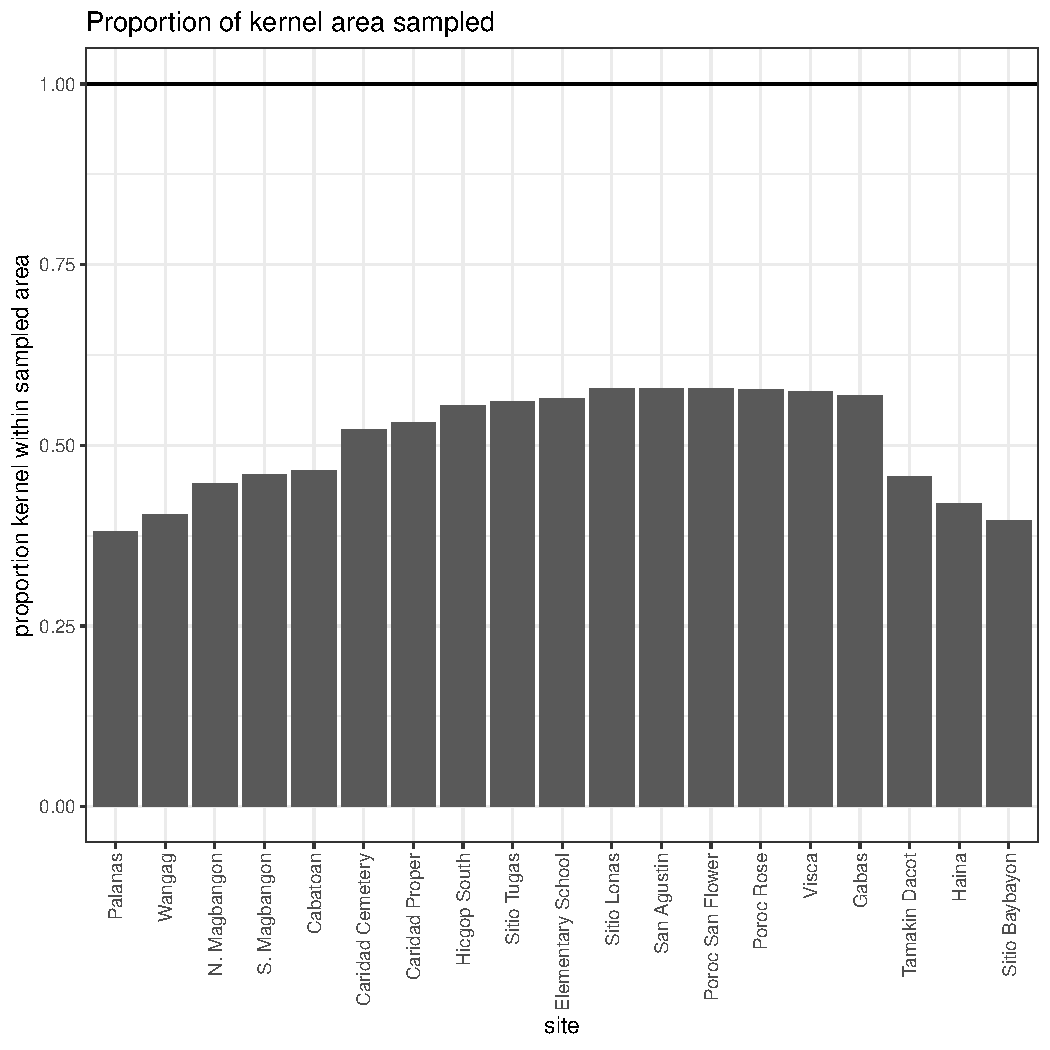
\includegraphics[width = 1.0\textwidth]{\detokenize{../Plots/FigureDrafts/Prop_of_kernel_area_sampled_by_site.pdf}}
	\caption{Proportion of the dispersal kernel area from the center of each site covered by our sampling. \label{APP_FIG_PropDispKernelAreaSampled}}
\end{figure}

\subsection{Probability of capturing a fish, from recapture dives} \label{APP_SEC_ProbR}

We use mark-recapture data from recapture dives done within a sampling season to estimate the probability of capturing a fish. During some of the sampling years (XX), portions of the sites were sampled again XX-XX weeks after the original sampling dives. We assume there is no mortality of tagged fish between the original sampling dives and the recapture dives because they are so close in time and that fish do not change their behavior or reponse to divers, so therefore assume that the probability of recapturing a fish is the same as the probablity of capturing a fish on a sample dive. For each recapture dive, we use GPS tracks of the divers to identify the anemones covered in the recapture dive and the set of PIT-tagged fish encountered on those anemones during the original sampling dives. We estimate the probability of capture $P_c$ as the number of tagged fish caught during the capture dive $m_2$ divided by the total number of fish caught on the recapture dive $n_2$: $P_c = \frac{m_2}{n_2}$. 

We use the mean $P_c$ across all 14 recapture dives, covering XX sites in 3 sampling seasons (2016, 2017, 2018), as our best estimate. Because there are so few recapture dives compared to the number of times we calculate the metrics to show the range of uncertainty, we represent the probability of capture as a distribution, rather than pulling directly from the values calculated for each recapture dive. The distribution of capture probabilities across the 14 dives is quite skewed so we represent it as a beta distribution, using the mean $\mu_{P_c}$ and variance $V_{P_c}$ of the set of 14 values to find the appropriate $\alpha_{P_c}$ and $\beta_{P_c}$ parameters, where 

\begin{eqnarray}
\alpha_{P_c} &=& (\frac{1-\mu_{P_c}}{V_{P_c}} - \frac{1}{\mu_{P_c}}) \mu_{P_c}^2 \\
\beta_{P_c} &=& \alpha_{\mu_{P_c}} \times \frac{1}{\mu_{P_c} - 1}. \label{APP_EQN_ProbCapBetaDistParams}  % Should I cite a source for this?
\end{eqnarray}

% Should I include a table of the recapture probs for each recapture dive, including site and year?

The mean of the individual capture probability values is $\mu_{P_c} = 0.56$, with variance $V_{P_c} = 0.069$, which gives beta distribution parameters $\alpha_{P_c} = 1.44$ and $\beta_{P_c} = 1.13$. We sample 1000 values from the beta distribution, then truncate the sample to only values larger than the lowest value of $P_c$ estimated in an individual dive (0.20), to avoid extremely low values that are sometimes sampled but are unrealistically low. We then sample with replacement from the truncated set to get a vector of values the length of the number of runs.

\newpage{}

\subsection{Full set of MARK models} \label{APP_MARKModels}
We consider the following set of models in MARK [\textit{Need to add in models}]:
\begin{table}
\begin{centering}
\begin{tabular}{|p{2in}|p{2.5in}|p{0.75in}|p{0.75in}|}
\hline 
\textbf{Model} & \textbf{Model description} & \textbf{AICc} & \textbf{dAICc} \\ \hline
& survival size, recapture size+distance & 3348.861 & 0 \\ \hline
& survival size, recapture distance & 3359.998 & -11.1371 \\ \hline
& survival constant, recapture distance & 3383.175 & 34.3141 \\ \hline
& survival constant, recapture size+distance & 3384.959 & 36.0981 \\ \hline
& survival time, recapture constant & 3408.342 & 59.4816 \\ \hline
& survival site, recapture constant & 3440.842 & 91.98112 \\ \hline
& survival site, recapture size+distance & 3440.842 & 91.98112 \\ \hline
& survival constant, recapture time & 3453.609 & 104.74839 \\ \hline
& survival size, recapture size & 3527.710 & 178.84940 \\ \hline
& survival constant, recapture constant & 3570.908 & 222.04690 \\ \hline
\end{tabular}
\end{centering}
\caption{}\label{APP_TAB_MARKmodels}
\end{table}

% Add plot of distances to anems in different years?
% Add plot of effect of size and distance on recapture probability?
\begin{figure}[H] % 4 relationships among parameters
	\centering
	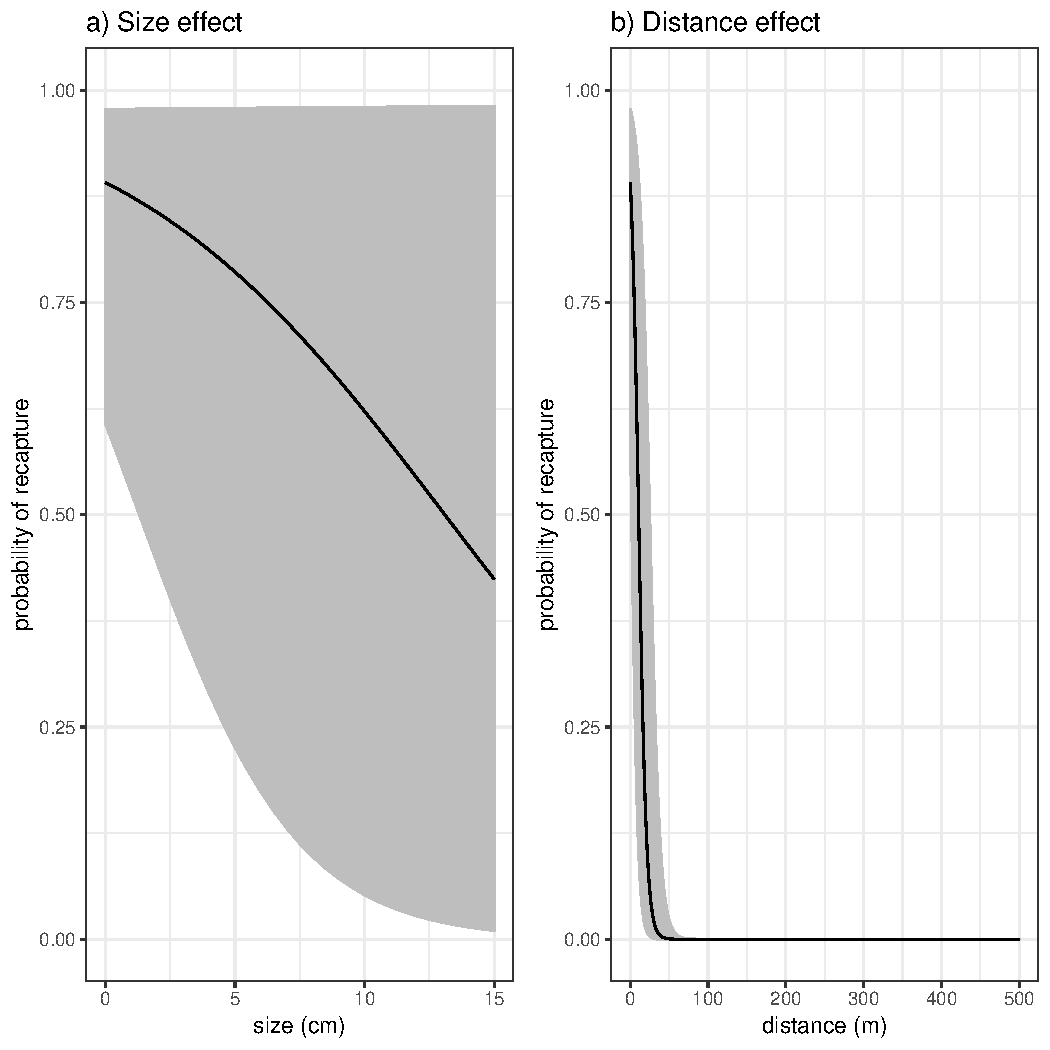
\includegraphics[width = 1.0\textwidth]{\detokenize{../Plots/FigureDrafts/Recapture_size_distance_effects.pdf}}
	\caption{Effects of a) fish size and b) minimum distance between divers and the anemone where the fish was first caught on the probability the fish will be recaptured, estimated along with survival in a mark-recapture analysis. Size has a slightly negative effect on the probability of recapture - larger fish are stronger swimmers and more likely to flee the anemone when divers approach. Distance also has a negative effect on recapture, as fish tend to stay close to their anemones and are not likely to be recaught if divers do not get close the their anemone. \label{APP_FIG_RecapSizeDistEffect}}
\end{figure}

\section{Uncertainty and sensitivity}

\subsection{What-if analyses}

To compare our replacement-based persistence results, which do not suggest that our sites make up a persistent metapopulation, with our abundance trends (Fig.\ \ref{FIG_FthroughTime}, which suggest that population abundances at our site have been relatively stable over our sampling period, we estimate recruits arriving at our sites per recruit there, regardless of the origin of the arriving recruits. We repeat our metric estimates but use all offspring genotyped at our sites, scaled by proportion habitat sampled within our sites $P_h$ and the probability of capturing a fish $P_c$, as our estimate of recruited tagged offspring. We see XXX, which means YYY. 

\paragraph{All genotyped offspring at our sites originated from our sites}

\begin{figure}[H] % Do we see replacement if we consider all recruits when looking at recuits-per-recruit?
	\centering
	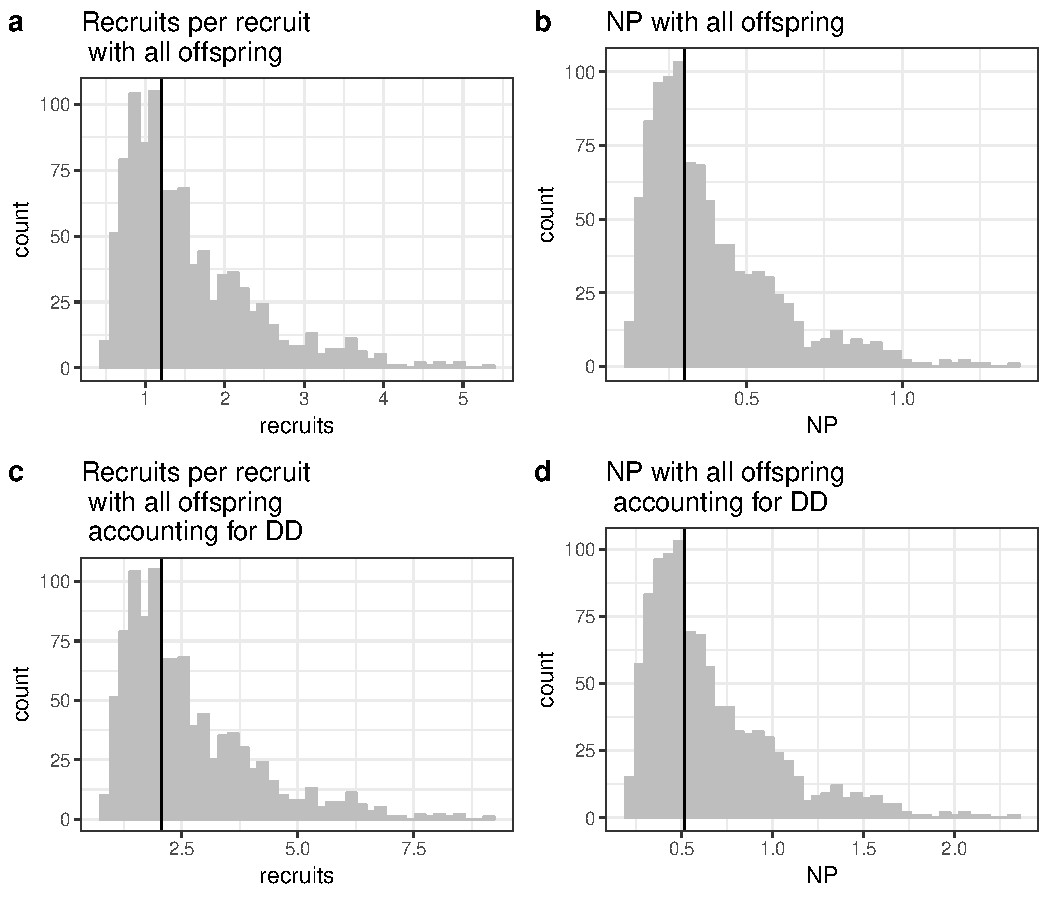
\includegraphics[width = 1.0\textwidth]{\detokenize{../Plots/PersistenceMetrics/Whatifs/LEP_R_and_NP_histograms_whatif_all_offspring.pdf}}
	\caption{a) Recruits per recruit when we consider all arriving recruits to have originated from our sites. b) Range of values of NP considering all arriving recruits to be offspring from our sites, with the best estimate in a black solid line. \label{APP_FIG_AllOffspringWhatIf}}
\end{figure}

\subsection{Sensitivity to parameters}

% Range of parameters used as input for uncertainty runs
\begin{figure}[H] % Range of parameter inputs for uncertainty runs
	\centering
	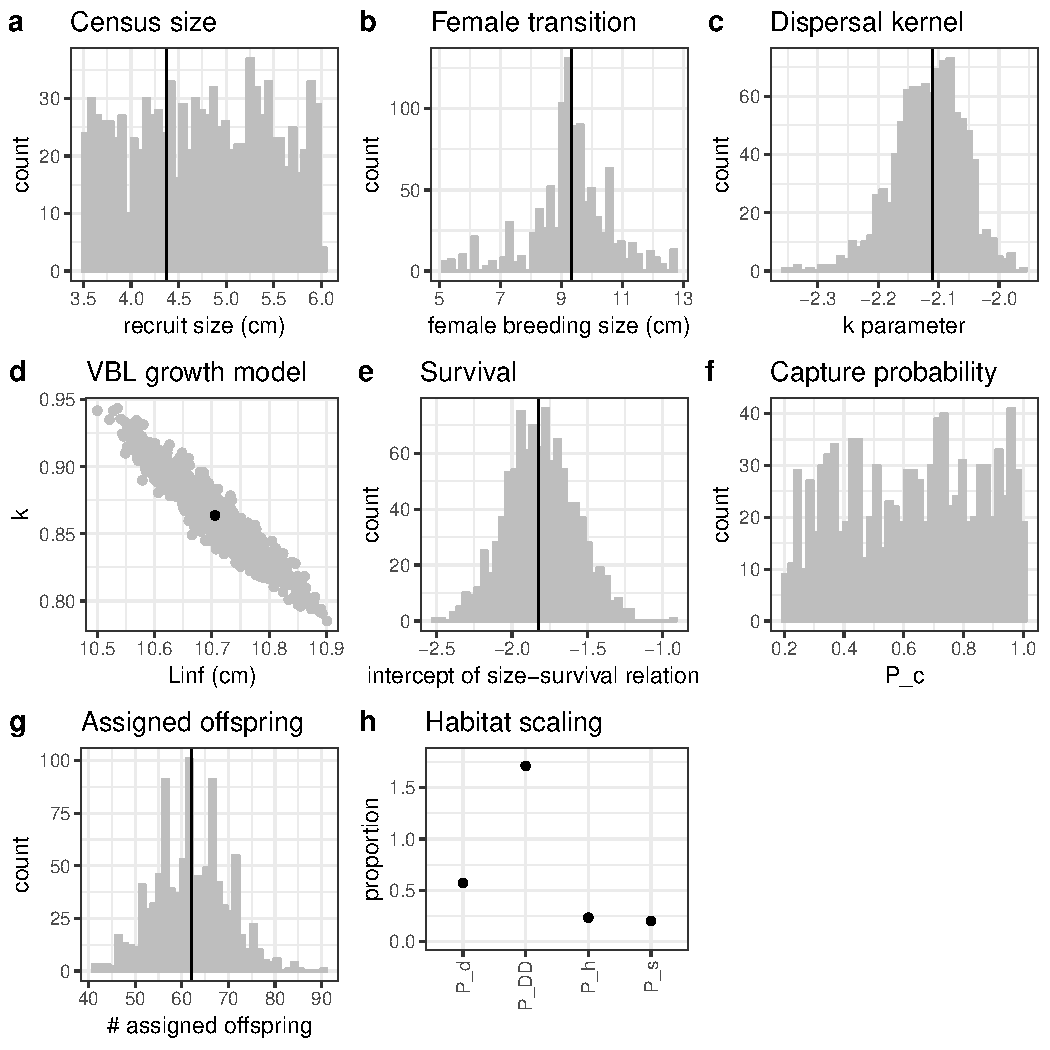
\includegraphics[width = 1.0\textwidth]{\detokenize{../Plots/FigureDrafts/Uncertainty_inputs.pdf}}
	\caption{Range of parameter inputs for uncertainty runs with all uncertainty included: a) $\text{size}_\text{recruit}$, the census size at which fish are considered to have recruited after egg-recruit survival occurs; b) $L_f$, the size at which fish transition from male to female and their reproductive output is included in the estimate of lifetime egg production (LEP); c) $k_d$, the scale parameter in the dispersal kernel; d) the parameters $L\infty$ and $K$ of the von Bertalanffy growth model; e) the intercept $b_\phi$ of the adult size-dependent survival relationship; f) $P_c$, the probability of capturing a fish; g) number of offspring assigned back to parents in the parentage analysis. \label{APP_FIG_UncertaintyInputs}}
\end{figure}

% Relationships among parameters

\begin{figure}[H] % 4 relationships among parameters
	\centering
	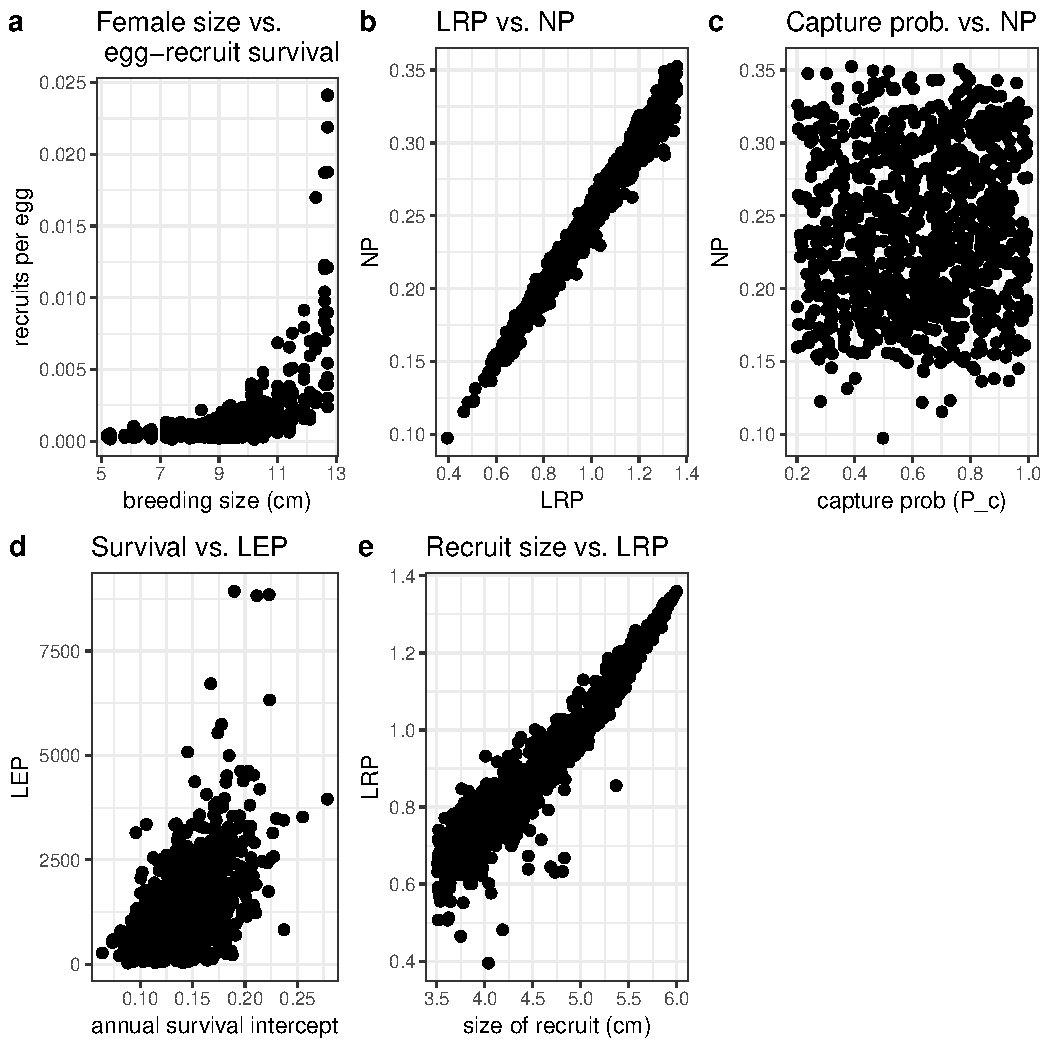
\includegraphics[width = 1.0\textwidth]{\detokenize{../Plots/FigureDrafts/Param_metric_relationships.pdf}}
	\caption{Relationships among parameters and metrics. a) We only count reproductive effort by fish in the female stage so the higher the transition size to breeding female, the fewer eggs parents are considered to produce, which increases the estiamted egg-recruit survival. b) LRP strongly affects NP by changing the number of potential recruits dispered through the connectivity matrix. c) The probability of capturing a fish does not have a clear relationship to NP. d) LEP is higher with higher survival estimates because fish are more likely to survive longer as reproducing adults. e) The size we consider to be a recruit marks the transition of mortality included in egg-recruit survival to mortality being captured by annual adult survival. Because we do not have the data to change egg-recruit survival to account for different recruit sizes, increasing the recruit size increases LRP by wrapping more mortality into the egg-recruit survival estimate, rather than LEP. \label{APP_FIG_ParamMetricRelationships}}
\end{figure} % Think about a better way to explain (e) and whether we should even include it.

\subsection{Effects of different types of uncertainty on metrics}

\paragraph{Lifetime egg production (LEP)}

Annual survival post-recruitment provides drives most of the uncertainty in LEP, as lower survivals keep fish from reaching and staying at large breeding sizes, with higher fecundity. The transition size to breeding female also drives uncertainty in LEP - the higher the transition size to female, the less time the fish has at a size where its reproduction is counted in LEP. 

\begin{figure}[H] % Uncertainty in LEP
	\centering
	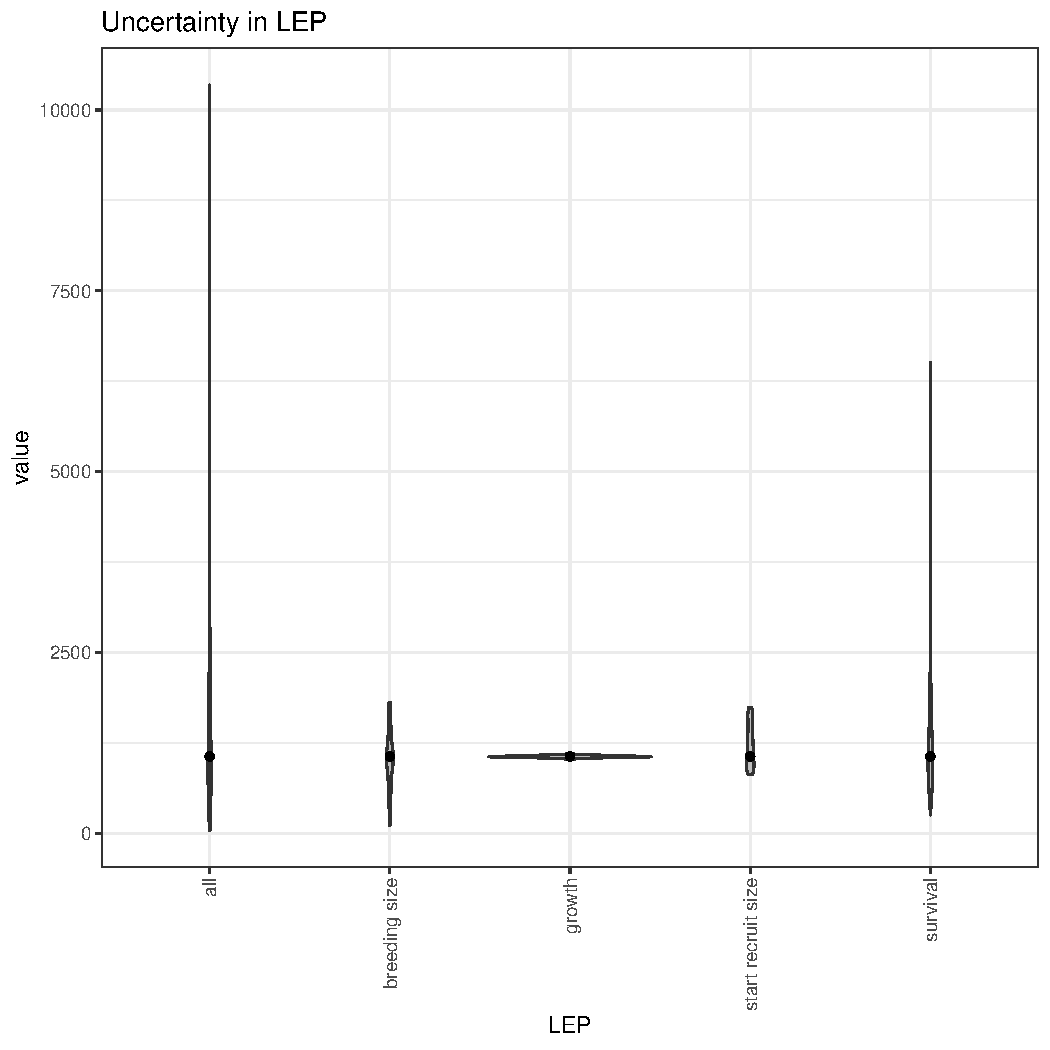
\includegraphics[width = 1.0\textwidth]{\detokenize{../Plots/FigureDrafts/LEP_uncertainty_breakdown.pdf}}
	\caption{The contribution of different sources of uncertainty in LEP. \label{APP_FIG_Uncertainty_LEP}}
\end{figure}

\paragraph{Lifetime recruit production (LRP)}

Most of the uncertainty in LRP comes from uncertainty in the size of a recruit. This is an artifact of our sampling, where we are unable to estimate egg-recruit survival differently to account for changes in the size of a recruit, so raising the size of a recruit reduces the mortality included in LRP without increasing the mortality included in egg-recruit survival, as it should in an ideal situation.

\begin{figure}[H] % Uncertainty in LEP_R - check plots, weird that assigned offspring and prob_r are just points (unless I don't understand how violins work? Shouldn't they be essentially horizonal lines if all runs have the same value, kind of like growth? Also, why does breeding size have such a different shape for LRP and LEP? Seems weird...)
	\centering
	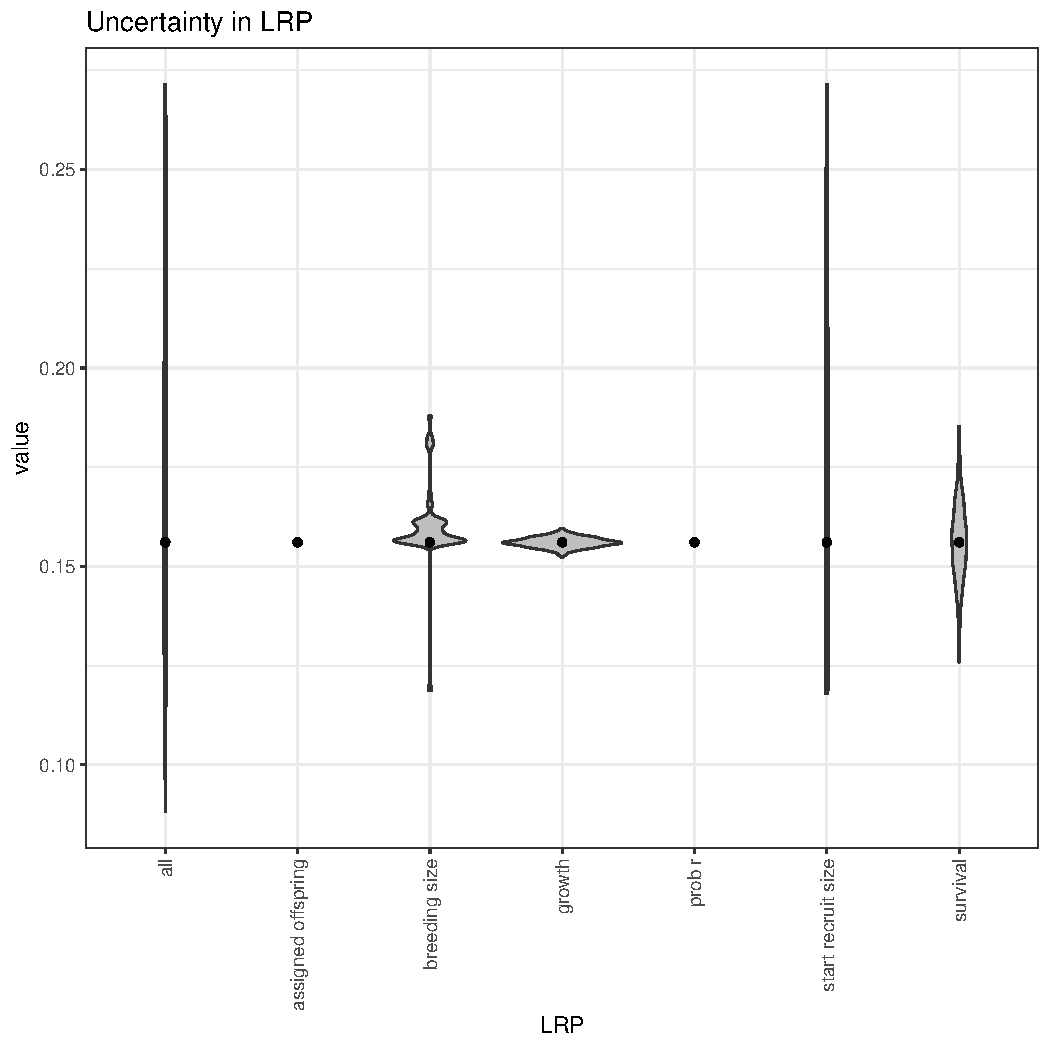
\includegraphics[width = 1.0\textwidth]{\detokenize{../Plots/FigureDrafts/LEP_R_uncertainty_breakdown.pdf}}
	\caption{The contribution of different sources of uncertainty in LRP. \label{APP_FIG_Uncertainty_LEP_R}}
\end{figure}

\begin{figure}[H] % Uncertainty in LEP_R with DD accounted for
	\centering
	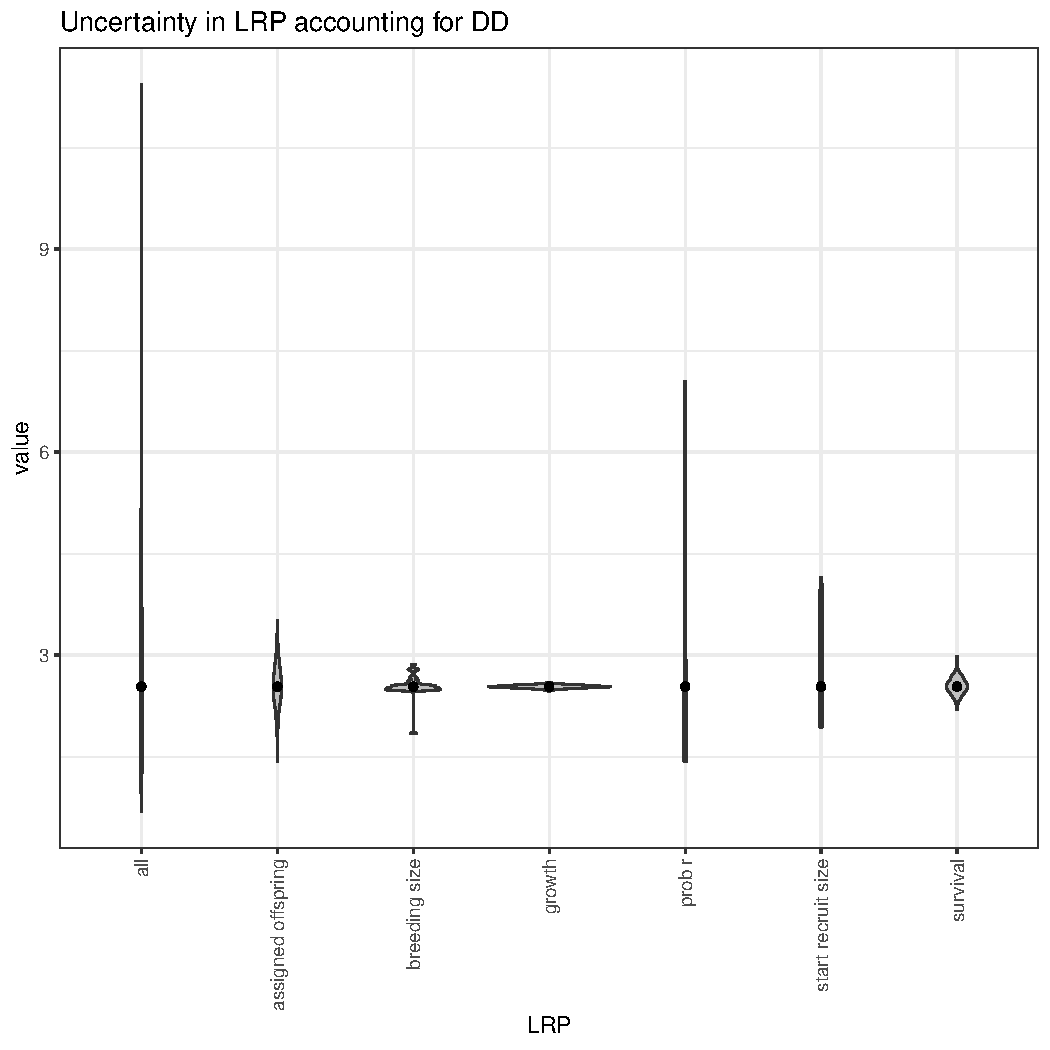
\includegraphics[width = 1.0\textwidth]{\detokenize{../Plots/FigureDrafts/LEP_R_uncertainty_breakdown_with_DD.pdf}}
	\caption{The contribution of different sources of uncertainty in LRP, when we account for density-dependence in egg-recruit survival. \label{APP_FIG_Uncertainty_LEP_R_DD}}
\end{figure}

\paragraph{Egg-recruit survival ($S_e$)}
\begin{figure}[H] % Uncertainty in recruits-per-egg
	\centering
	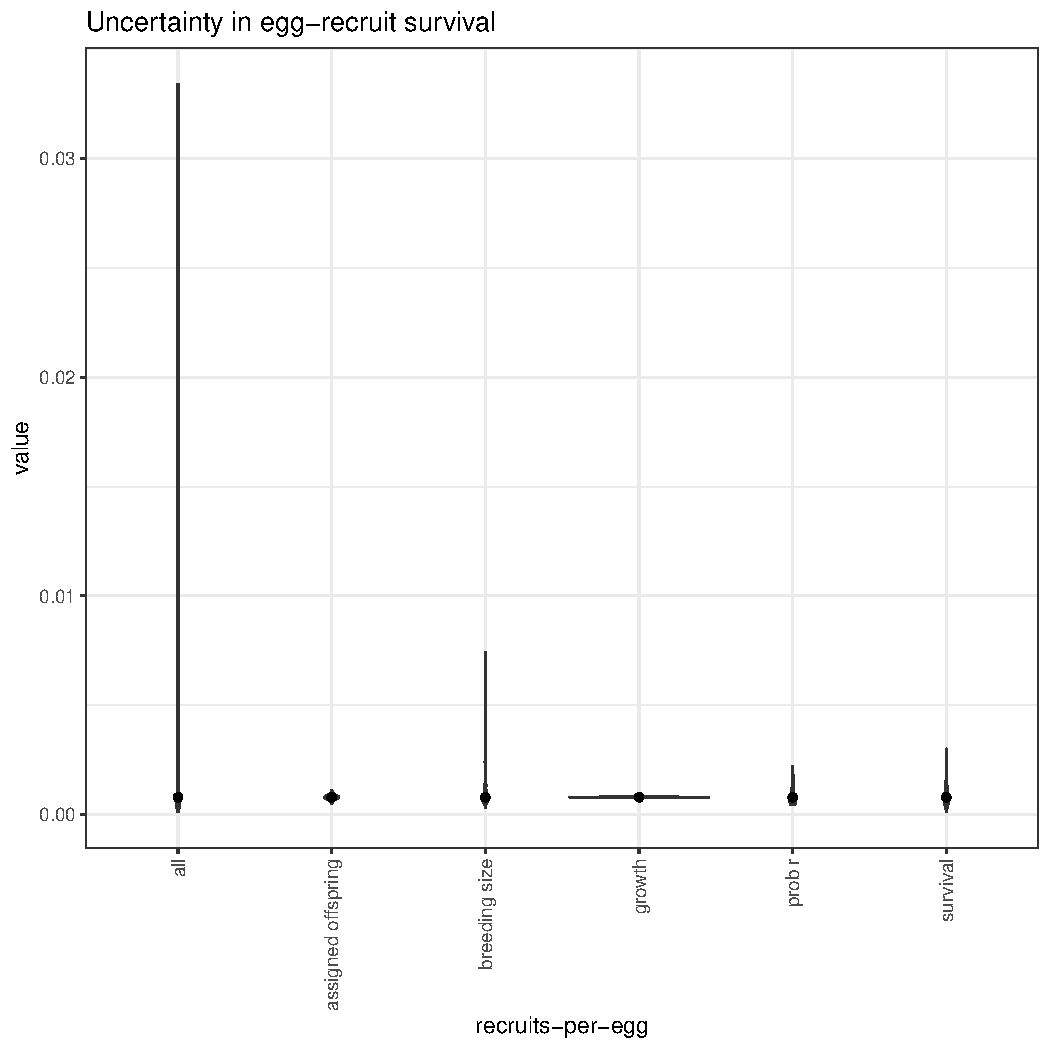
\includegraphics[width = 1.0\textwidth]{\detokenize{../Plots/FigureDrafts/RperE_uncertainty_breakdown.pdf}}
	\caption{The contribution of different sources of uncertainty in egg-recruit survival. \label{APP_FIG_Uncertainty_RperE}}
\end{figure}

\begin{figure}[H] % Uncertainty in recruits-per-egg with DD accounted for
	\centering
	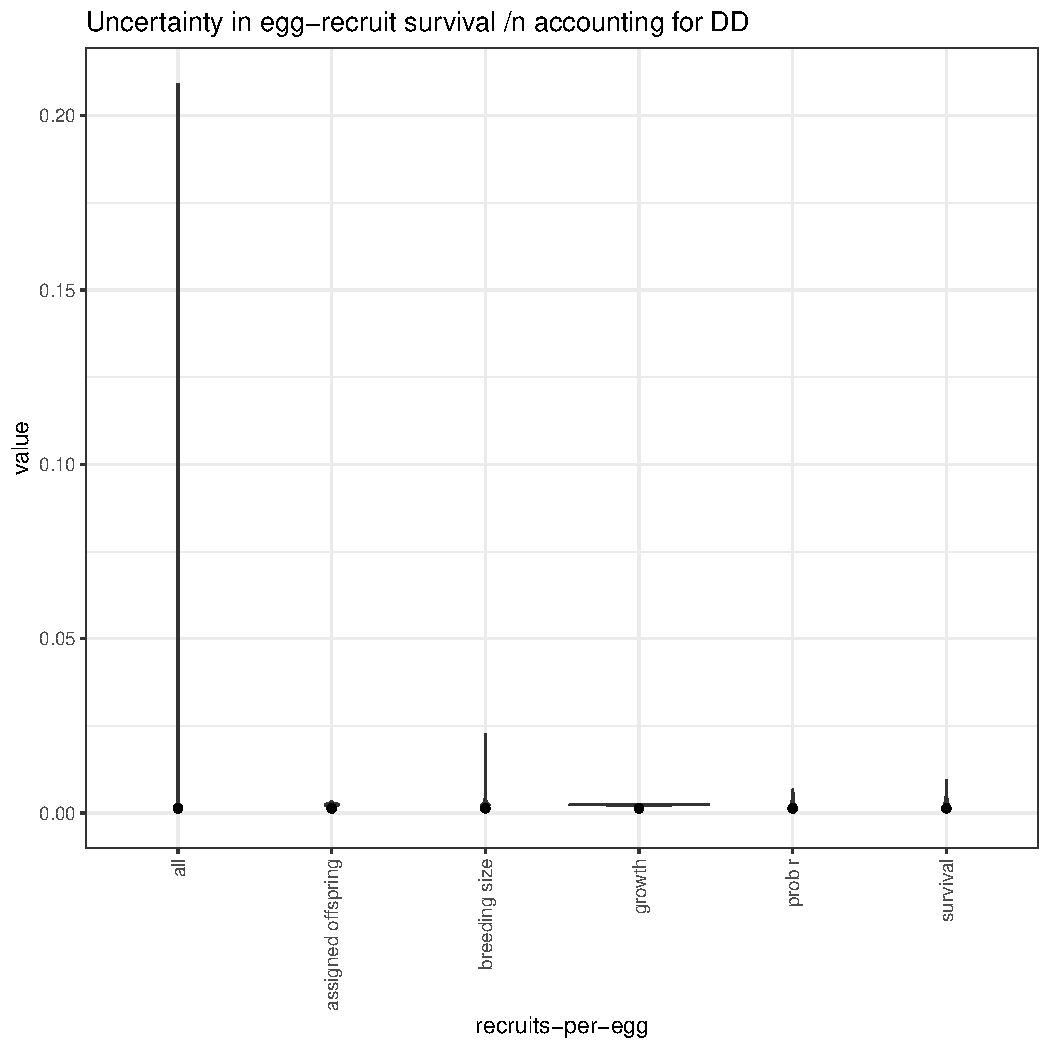
\includegraphics[width = 1.0\textwidth]{\detokenize{../Plots/FigureDrafts/RperE_uncertainty_breakdown_DD.pdf}}
	\caption{The contribution of different sources of uncertainty in egg-recruit survival when we account for density-dependence in egg-recruit survival. \label{APP_FIG_Uncertainty_RperE_DD}}
\end{figure}

\paragraph{Network persistence (NP)}
\begin{figure}[H] % Uncertainty in NP
	\centering
	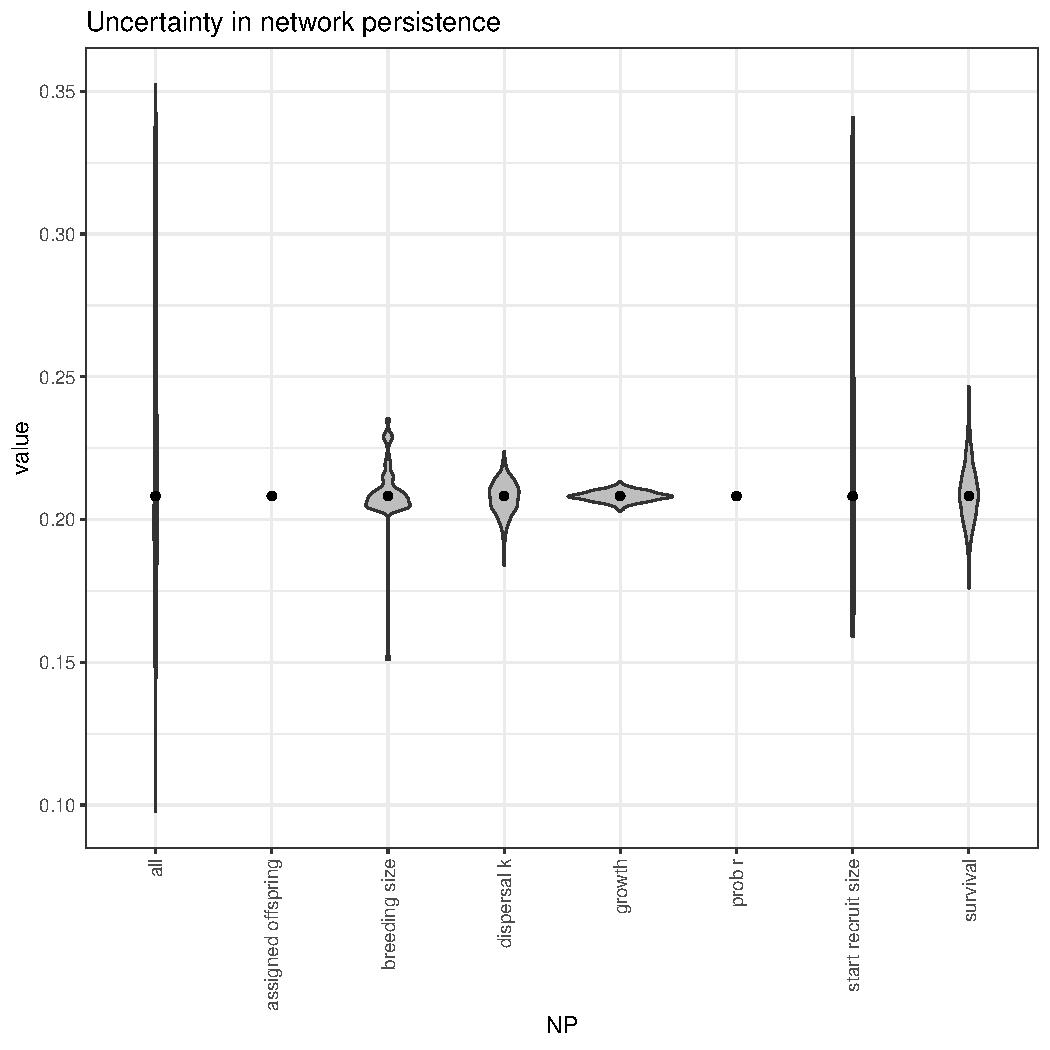
\includegraphics[width = 1.0\textwidth]{\detokenize{../Plots/FigureDrafts/NP_uncertainty_breakdown.pdf}}
	\caption{The contribution of different sources of uncertainty in NP. \label{APP_FIG_Uncertainty_NP}}
\end{figure}

\begin{figure}[H] % Uncertainty in NP with DD accounted for
	\centering
	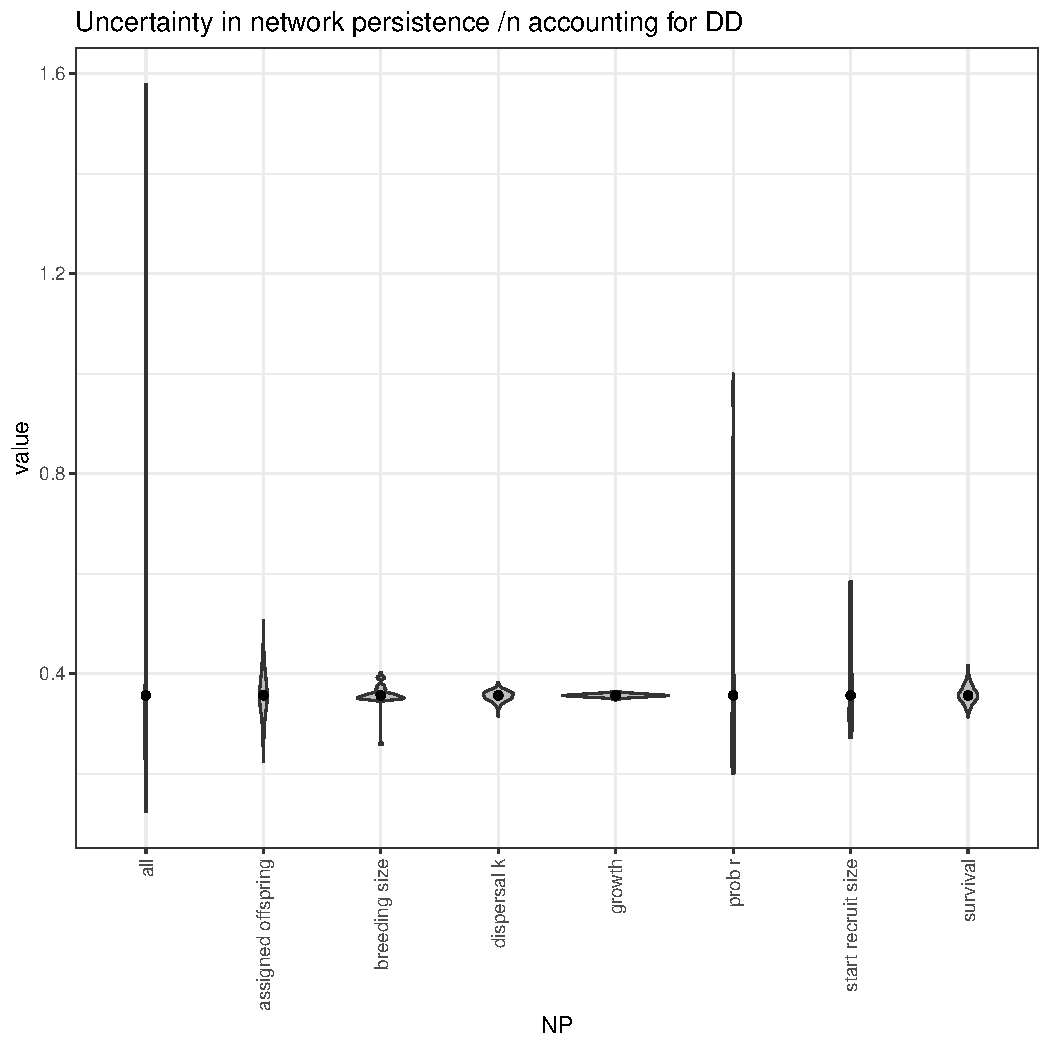
\includegraphics[width = 1.0\textwidth]{\detokenize{../Plots/FigureDrafts/NP_uncertainty_breakdown_DD.pdf}}
	\caption{The contribution of different sources of uncertainty in NP when we account for density-dependence in egg-recruit survival. \label{APP_FIG_Uncertainty_NP_DD}}
\end{figure}

\newpage{}

%\bibliography{../../../BibTexReferences}
\bibliography{BibTexReferences}
\bibliographystyle{plainnat}

\end{document}